\documentclass[a4paper, 10pt]{article}

\usepackage{graphicx} %%Good primer on this see:  https://www.youtube.com/watch?v=Ax9RCvjpI8E
\usepackage{subcaption}

\usepackage{geometry} %%To set basic page parameters. See also: https://www.overleaf.com/learn/latex/Page_size_and_margins
\geometry{a4paper, portrait, margin=1in}

%%Use this when you want to change colors eventually: https://tex.stackexchange.com/questions/75667/change-colour-on-chapter-section-headings-lyx

%%This is a function I found on stack overflow when I looked up
%%'How can I change the margins for only part of the text?'
\def\changemargin#1#2{\list{}{\rightmargin#2\leftmargin#1}\item[]} 
\let\endchangemargin=\endlist 
%%Use it sparingly.

\renewcommand \thesection {\Alph{section}} %%Defines section numberings (A.1.1, etc)

\begin{document}

\begin{titlepage}

	\begin{figure}[h]
		\centering
		
\includegraphics[scale=.8]{Photos/HackRoverlogolofi}
	\end{figure}

	\begin{center}
		\vspace*{1cm}
	
		\Huge
		\textbf{HackRover}\\[10pt]
	
	
		\large
		\textbf{Capstone MegaDoc}\\[40pt]

		\begin{changemargin}{10pt}{10pt} 
		\begin{center}
		\normalsize
		Justin Heinzig, Danny Kha, Jacob Park
	
		Advisor; Mentor; Sponsor: Pierre Mourad\\[150pt]
		\end{center}
		\end{changemargin}
	\end{center}
	
	\begin{figure}[h]
		\centering
		
\includegraphics[scale=.8]{Photos/UWLogo}
	\end{figure}		
	
\end{titlepage}

\pagebreak{}

\tableofcontents

\pagebreak{}

\section*{Foreward}
	\subsection*{Abstract}
	----This is a meta section about how this paper is ordered.	
	
	\subsection*{Executive Summary}
	HackRover is a cyber-defense-based student research project aimed at making, breaking, and hacking mobile platforms, encompassing rovers, drones, and anything that moves. Our goal is to practice and develop skills to help defend our increasingly connected world of embedded systems, where the safety of people and communities is being placed in the hands of autonomous machines.
	
	Our plan is to pioneer a new type of hacking competition - named the HackRovoer Autonomous Robotics Competition (HARC) - where participants attempt to infiltrate self-driving rovers and collect round-winning information. There is no hackathon in the world that is centered around autonomous machines, yet according to a 2019 Global Autonomous Driving Industry Outlook report, 1 in 4 cars are expected to have autonomous capabilities by 2030. The competition we're creating isn't exclusive to UW Bothell, as tentatively schools around the globe can set up chapters. Succeeding in creating such an event would result in an excellent pedegogical tool. 
	
	Each iteration of the competition the theme changes, which influences competing rovers' designs, puzzles and props within the competition, and game rules. This iteration's theme is disaster relief; participants are tasked with designing rovers which find themselves in disasters like collapsed buildings or tornado paths. They'll build rovers for a hypothetical company which would sell to local governments and emergency services in disaster prone-regions. Rovers would provide mostly scouting and minimal medical function, either/both seeking out victims (such as under rubble) or/and dispensing minimal medical aid. Obviously the competition is yet to exist officially, so we act as a lone team following the themes set for ourselves. 
	
	This year we completed the construction of a disaster rover (first iteration), nicknamed Mimir, as well the competition puzzle panel, a prop which the rover interacts with. The rover we designed consists of three tiers stacked onto a drive base: the bottom tier houses micro-controllers and electronic power distribution; the middle tier houses the microcomputer and communication devices; and the top tier houses the LiDAR camera system and its control Stewart platform. The puzzle panel contains small electromechanical devices mounted by velcro to a velcro-clad, wooden puzzle; these devices are currently interfaced by an Arduino Mega and custom design, PCB power distribution system (PDS). See below are the two devices completed this quarter.

	--------------------ADD THE IMAGES
	
	------------------------------------------
	
\pagebreak

	\subsection*{Project Requirement Documentation}
	The disaster rover we're building must be debris resistant and capable of traversing non uniform terrain. Functionally it must be controllable over a wireless connection (network satellite or otherwise) with a standard XBox gaming controller or keyboard. It should send any and all sensor data back through the connection to a browser-based GUI; this quarter the data will at minimum include LiDAR camera images. Internally the rover needs: (1) a PDS to provide 12V and 5V through various means, (2) a central command microcomputer capable of making all necessary high level logical decisions, (3) microcontrollers capable of communicating control commands to the rover drive train and LiDAR's position control device, and (4) networking devices enabling the rover to be operated wirelessly. The PDS should provide clean energy to motors and logical devices simultaneously, as well as present additional 'ports' for future devices and add-ons. The central command microcomputer should be capable of interfacing with all control components, operating at a high level (with the GUI and user), and centralizing control. The microcontrollers should forward information to the control mechanisms (servos, motor controllers, etc) from the central microcomputer. The networking devices must provide switch functionality, to interconnect devices within the rover, routing functionnality, to interface the rover with outside networking, and wireless access.
	
	The puzzle panels for the competition should emphasize easy engineering: mechanical, electrical, and computer. Mechanically, devices should be easily and reliably mounted and interfaced on a flat board. Options for configuration should be provided for maximum puzzle design creativity. Electrically, all components should have access to clean power through a simple panel PDS without significantly effecting the power recieved by other components. Signals must be sent into and out from an Arduino central microcontroller with ease. Computer-wise, components should have code libraries created for easily prototyping and producing a myriad of puzzle arrangements. Students unfamiliar with programming should be able to learn and create with short lead time, and not have to worry about seeking out libraries or software components for themselves. 
	
\pagebreak

\section{Design Strategy}
	\subsection{User Insights and Research} 
		\subsubsection{Consumer Journey Map}
		The unique nature of our project makes consumer analysis difficult, as product consumption occurs at multiple levels: faculty, students, companies, disaster responders, etc. Here we'll speak lightly of most and provide consumer journey maps for students and disaster responders: the key subjects of our capstone project.
		
		When structuring education, university faculty seek useful pedegogical tools; such tools will provide  interdisciplinary education, equip students with life skills, and possibly generate research/products that enrich the name and wealth of the school. Students, specifically engineering ones, look to develop their skills while in school through participation in clubs, projects, and research. They're often pulled in many directions as their educational appetite is wide but options are slim/focused.
		
		%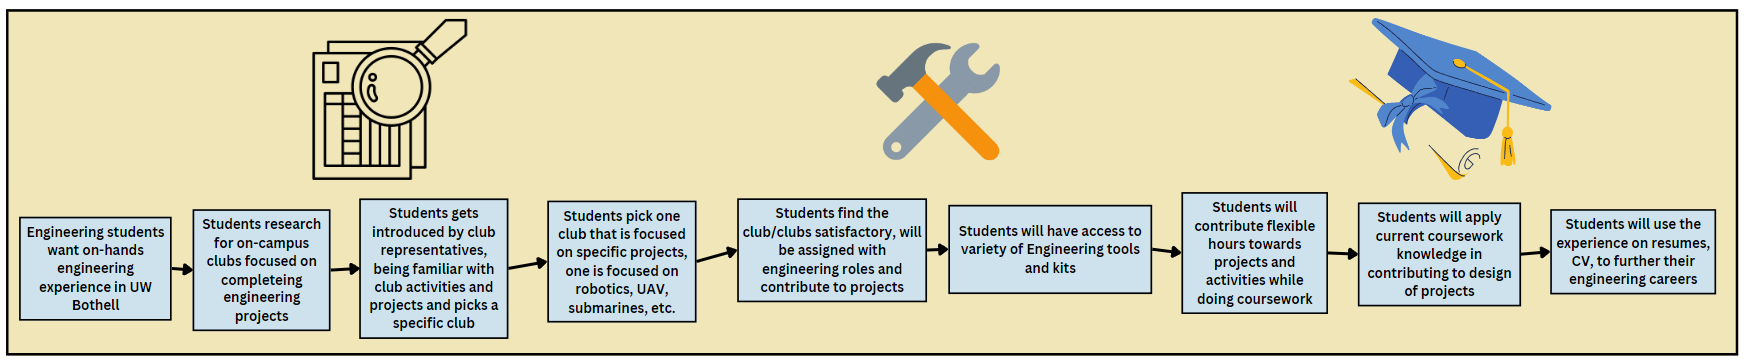
\includegraphics[scale=0.4]{Photos/Student Consumer Map}
		
		The student should look for extracurriculars, see options, have to pick an option, each option should have different range of benefits.
		
		Seen above is a student consumer map cataloging the journey a student experiences as they seek extracurricular, educational activities which empower them. A key takeaway is that the student is limited by time and must select one club with a narrow purpose. Further, these clubs demand a wealth of previous knowledge and experience to properly participate, raising the bar to entry. Broadening the scope of work for any given organization and lowering the bar to entry are obvious improvements.
		
		Robotic companies that develop disaster rovers are limited by the opportunities available to them and niche of their field. Disaster relief is a philanthropic endeavor for the most part, where the only money to  be made is from tech savvy local governments (an already fickle customer) or when disaster relief can be re-purposed as a virtuous advertisement. Minimal money exists in prize form through government sponsored competitions or events, like DARPA's disaster relief competition. Beyond monetary opportunity, research is hard to come by; like an ouroboros, the lack of monetary gain causes people to ignore robotics research in disaster relief. This makes constructing disaster relief systems difficult all around. A disaster responder's role all of this makes R\& D even more difficult, as relying on robotic systems is a difficult and risky endeavor. You're never sure when a disaster will strike, and circumstances are unique each time. As a responder you must delegate quickly and make use of limited resources in saving as many lives and limiting damage as possible. Rovers are dependent on a human operator as well as some uptime; further, their operation needs to be clean and quick to permit a disaster responder to complete the same or better task without major risks.
		
		%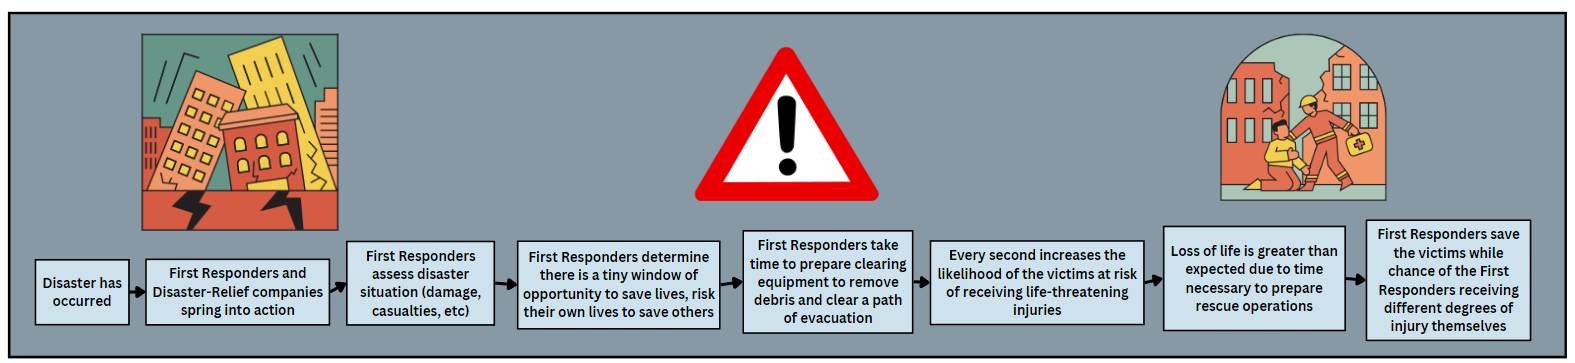
\includegraphics[scale=0.45]{Photos/Disaster Consumer Map}		
		
		The disaster responder should be presented with a disaster, have to quickly assess damages, delegate  resources in a timely manner, save people, make risks. Possibly emphasize the risks they might take, and talk about the time it takes to accomplish their goal. 
		
		Seen above is a disaster responder consumer map cataloguing their response to a generic disaster event. Of emphasis is the risk to responder's life, a time crunch, and quick decision making with limited resources and information. Systems or methods that might remove the human operator from danger, improve operation efficiency, and maximize life-saving information and resource use are obvious improvements.
		
		
		\subsubsection{Stakeholder Framing}		
			\begin{itemize}
			\item
			\textbf{Stakeholder:} \emph{Government Relief Organizers:} The bottom line of these individuals is effective distribution of force and resources; inability to do this casts doubt on their ability. Any cost effective solution which improves how they distribute resources, or reduces resources needed will be a boon to them. 		
			
			\item
			\textbf{Stakeholder:} \emph{Disaster Relief Operators:} Like the government organizers above, these individuals need to manage a swath of resources; albeit smaller, with more attention. Tools that can sub in for more expensive resources, have shorter uptimes, improve information gathering, accomplish rescue, and maximize human life (operator or victim) are beneficial.
			
			\item
			\textbf{Stakeholder:} \emph{UW Bothell Students:} UW Students are the primary beneficiaries of our product. Prior we made clear the intent to create a product that serves UW Bothell students first and foremost, and whose reprocussive effects are benefits to disaster response. Providing students with extracurricular engineering activities that are easy to get into while simultaneously serving broad interests will nix the problem of narrow-focus clubs with steep learning curves. 
			
			\item
			\textbf{Stakeholder:} \emph{UW Capstone Core Team:} Our organization already exists, but the product we create will have bearing on our success. The ability to serve a  need within the school has direct correlates to further funding and participation.

			\item
			\textbf{Stakeholder:} \emph{Pierre Mourad:} Pierre derives benefits from the product in the form of reputation of his person, outreach for access to students (for other projects potentially), and access to robotics systems. Our performance in this capstone cycle will affect trust in his decisions.
			
			\item
			\textbf{Stakeholder:} \emph{UW Faculty:} Like Pierre, the UW faculty has a stake in this project. They've provided plenty of resources and space which might be used for something else. Further, a successful project might provide a powerful pedagogical tool in the future.

			\item
			\textbf{Stakeholder:} \emph{UW Student Technology Fund:} The STF is the primary contributor to our organization, providing more than 3000 dollars in hardware technology. The exchange of this technology was meaningful use, future requests need to be paired with demonstration of this good use.
			\end{itemize}
			
			
		\subsubsection{User Scenarios and Personas}
		\subsubsection*{Three Personas:}
		\begin{itemize}
			\item
			
			\emph{UW Student seeking a club} A prototypical UW engineering student seeking out extracurriculars to further their knowledge of mechanical, electrical, and/or computer  engineering. 
			
			\item
			\emph{UW Faculty seeking new educational resource} A UW faculty member desiring to contribute to the education of their students while generating value within the school.
			
			\item
			\emph{Disaster responder} A diasaster responder on the ground attempting to respond to an earthquake that resulted in the collapse of multiple buildings with people inside.
		\end{itemize}
		
		
		\subsubsection*{Scenarios:}
		\begin{itemize}
			\item
			A students looks at a roster of available clubs and organizations to participate in with the aim of furthering their engineering ability in multiple fields and equipping them with industry-standard skills. They're met with a limited selection containing clubs that exist but don't operate well, and others which are popular; all of these clubs have a niche focus that forces the student to sacrifice some of their interests if they invest their time. The student picks a popular club and is met with a great amount of competition and steep learning curve. Everyone wants to contribute and do something cool, but resources are limited, so competition ensues. To stand out the student  must struggle to learn a massive amount of content; by the end their skills may no longer  be useful. Trying to latch onto existing projects within the club is difficult because documentation is sparse and the student can't understand decisions that were made. These circumstances aren't different for others so the project sits in gridlock: afraid to move forward in case precious resources are destroyed during the process of improvement, and a lack of confidence in how to move forward, since decisions require immennse background knowledge (which isn't well documented). The student spends most of their time jumping hurdles just to do minimal meaningful engineering, get discouraged, and use the club as a resume filler.

			\item
			A faculty member has to balance their desire to improve their students lives with forwarding their own career. They could create a product which is a horrible pedagogical tool and hyper-focuses the education of their student, but which benefits their own reputation and school image. Alternatively they create product which is great for educating students, but doesn't draw any attention or produce meaningful results/research. 
			
			\item
			A disaster responder is provided a small troop of men to command with limited expensive resources to save as many lives as possible in a short amount of time. If they spend too much time deliberating, hundreds may be crushed or suffocated under rubble; if they act too quickly manpower and resources will be spent inefficiently, hundreds may still die. Information collection and action must also be balanced. Any work they do also places their own team-members lives' at risk.
		\end{itemize}
		
		\subsubsection*{One Scenario Environment}
		The environment of focus is the disaster responder since it's scenario which motivates most development decisions within the project. The student is important but accessory to the disaster responder. We've repeatedly emphasized above the time and resource intensive environment responders participate in, increased consideration to human life, and limited information. Furthermore, disaster responders are beholden to government organizers who provide resources for disaster response. Despite being the users of our product, the responders must be able to convince higher ups the acquisition is sensible and cost-effective.

		\subsubsection{User Insight Report}
		\textbf{UW students} need a product that address their lack of interdisciplinary, extracurricullar activities. acitivities provided by the product must be friendly to students of any educational background and not require them to climb a steep learning curve; documentation of past activities should be plenty yet easy to read. Clerical work should be minimized, while real engineering work is maximized. Any participation should result in industry skills being learned.
		
		\textbf{UW faculty} members need a product that is both pedagogically developed and useful for producing reputable work and/or research. 		
		
		A given of our capstone is the development of some rover that addresses disaster responders' issues, beyond additional product components which address UW students' needs. We've made it very clear that \textbf{disaster responders} need a rover design that's cost effective, as to convince government organizers of acquisition; has a short up-time and is easy to control, to maximize efficiency; and, can provide vital information, to streamline rescue missions and better distribute resources.
		
		A few meetings with our sponsor, Prof. Pierre Mourad, shed light on both the school environment and state of disaster relief robotics. It seems Bothell suffers from limited engineering extracurriculars, many of which are too narrow (as per our previous mention); the only solid `rover' project is TrickFire, which sees heavy member competition. Furthermore, few pedagogical tools exist for students; many try to learn through clubs, but those often require extensive background understanding. Pierre Mourad  also discussed his understanding of disaster relief rover design: companies would rather send a specifically configured rover into the situation substitute for a responder, but close by. Rovers would need to be easily configurable or provide enough data under small up-time to legitimize their use in the field. Rovers should also have some autonomous  function so they don't have to be babysat by their operators.

	\subsection{Problem Understanding}
		\subsubsection{Product Assumptions}
			\begin{itemize}
			\item
			For UW Students: A product that addresses their lack of interdisciplinary, beginner-friendly extracurriculars, which improves their education, equips them with industry-standard skills, and provides an outlet for creative design. 
				
			\item
			For UW Faculty: A product that addresses their lack of pedagogical tools \& reputable student projects, providing benefit in the form of an excellent learning tool they might direct students towards while simultaneously generating projects that advance the school's reputation.
		
			\item		
			For disaster responders: A product that addresses their time \& resource constraints while responding to disasters, and concern for human life, by providing life-saving information (or even saving lives) with little up time, small cost to direct supervisors, and ease-of-use. 
			\end{itemize}


		\subsubsection{Functional Assumptions}
			\begin{itemize}
			\item 
			For UW Students: A product that addresses their lack of interdisciplinary, beginner-friendly extracurriculars, which improves their education, equips them with industry-standard skills, and provides an outlet for creative design, via that product's pedagogical methods, emphasis on industry practice, and interesting activities. 
		
			\item		
			For UW Faculty: A product that addresses their lack of pedagogical tools \& reputable student projects, providing benefit in the form of an excellent learning tool they might direct students towards while simultaneously generating projects that advance the school's reputation, via that product's pedagogical methods, and activities that generate documentation and design research. 
		
			\item
			For disaster responders: A product that addresses their time \& resource constraints while responding to disasters, and concern for human life, by providing life-saving information (or even saving lives) with little up time, small cost to direct supervisors, and ease-of-use, via that product's data collection systems, simple configuration, cheap yet robust construction, and intuitive controls.	
			\end{itemize}
		

		\subsubsection{High Level Usability Constraints}
			\begin{itemize}
			\item 
			For UW Students: An accessible, well funded, educational product that addresses their lack of interdisciplinary, beginner-friendly extracurriculars, which improves their education, equips them with industry-standard skills, and provides an outlet for creative design, via that product's pedagogical methods, emphasis on industry practice, and interesting activities. 
		
			\item		
			For UW Faculty: A well-documented, effectively managed, economically efficient educational product that addresses their lack of pedagogical tools \& reputable student projects, providing benefit in the form of an excellent learning tool they might direct students towards while simultaneously generating projects that advance the school's reputation, via that product's pedagogical methods, and activities that generate documentation and design research. 
		
			\item
			For disaster responders: A short up-time, easy-to-use product that addresses their time \& resource constraints while responding to disasters, and concern for human life, by providing life-saving information (or even saving lives), and small cost to direct supervisors, via that product's data collection systems, simple configuration, cheap yet robust construction, and intuitive controls.	
			\end{itemize}

		\subsubsection{Final Need Statement and User Outcomes}
		\textit{A short up-time, easy-to-use product which considers the time \& resource constraints of disaster responders while providing life-saving information. The product will certainly be a rover, easy to configure and operate, cheap, and with robust data collection systems, altogether easy to control. The entire rover will be developed within the context of an undergraduate robotics competition, where competition props (mostly electromechanical) and guidelines will serve as pedagogical tools, and all student activities will be documented according to industry standards, (documentation technology and formats).}
	
		This is a tricky two-part needs statement: (1) the rover portion of the product for the disaster responders, and (2) the product satisfying the needs of the students. The aim was to direct student efforts and learning to the construction of the physical product; this directed effort is accomplished through the pedagogical tool which is the competition. 

		\subsubsection{Hypothesis Statement}
		For the disaster responders, the product is obviously going to be a rover. For simplicity of prototyping we're going to design a earthquake disaster response rover. We believe a system which is dust and rubble resistant, capable of semi-autonomous action, collecting and relaying data, cheap to manufacture, and easy/quick to setup will help in information collection and decision making for disaster response teams, and potentially serve functions traditionally held by human responders, preserving human life. 
		
		This physical product will be prototyped within some educational setting which acts as the abstract, student-serving component of the product. We're the educational setting is going to be a competition, but the specifics of the guidelines are unclear as of now. The competition would be managed by our organization, which is both a club and capstone. 

		\subsubsection{Possible Inventions and Business Model}
		\subsubsection*{Possible Inventions:}
		Current systems for disaster relief are overly-expensive, shallow attempts at a design that jerry-rig existing structures/systems to solve issues of disaster relief. What’s more is that these systems rarely provide meaningful help, have large uptimes, or return limited data back. For example, aerial systems show snapshots from a bird's eye view, but little more; they're expensive to acquire, time-consuming to deploy, and require a skilled operator. Some might argue that visual feedback is enough to trace access paths and gauge the scope of the damage, but it gives a limited understanding of victim locations, danger points, etc. Another example: most land rovers - despite being capable in their locomotion - return limited useful sensor data (compared to drones), and the current state of actuative technology is limited. The biggest thwart to effective disaster technology, however, is the context in which it's developed. Frequently made by heavy industry tech giants, the return on investment is minimal and opportunity costs are great; to them, the effort is best served elsewhere. The only place to turn to, then, is University Students who are willing and wanting to work for the low cost of a good resume and contribution to society. Here effective organizations need to be made to mobilize their talents into the creation of disaster relief robots; the best scenario is a robotics competition. Most existing competitions see students participating in events that see them designing rovers tailored to useless/limiting activities, or just working with a confining kit and no creative freedom at all. Though some break the mold, they're few and far in between, and none focus on disaster relief. To further robotic, disaster relief tech, effective student organizations must be created.
		
		The first obvious 'invention' of this capstone is a disaster relief-oriented competition, which we call the HackRover Autonomous Robotics Competition (HARC). Traditionally it existed to provide an outlet for interdisciplinary engineering practice and an exploration of IoT; but, as the competition itself has no context there is a point for improvement. This new iteration emphasizes the creation of puzzle panels with elements and a point system that inspires the design of autonomous systems with capable actuation, computer vision and vision processing, capable locomotion, short up-time, easy configuration, and quick access.
	
		There are some hacking competitions, and even disaster robotics competitions, (such as the one hosted by DARPA); but, all of these are largely philanthropic endeavors. Certainly we have the UW system as our foundation, and will likely recieve meaningful funding from them, but this only offsets the cost of physical hardware they deem absolutely necessary. To make this organization really stand out and be financially viable we theroized a few `inventions': (1) a payment scheme for participants, (2) providing design favors to local companies in exchange for funding, and (3) providing student research favors to local companies in exchange for funding. The first is obvious, participants in the competition will pay a fee, but this will likely only offset food, advertising, and more. The second and third see UW students dedicating physical design efforts, or research efforts proportional to the money gifted by a local company. For example, say that Boeing wants a unique end effector which performs a task they might see in their factory, and donates \$4,000, while Lowes wants a software architecture reflective of potential AGVs in their warehouse and donates \$6,000; HackRover may or may not form capstone inspired by these requests, but would dedicate 40\% of their extra manpower to Boeing's desires, and 60\% extra to Lowes.
	
	----ADD DARPA SPLASH

		The second main invention is a modular rover framework. In the past, the biggest hurdle for all robotic systems has been the software architecture, which must be uniquely tailored to the hardware being employed. With the help of some middleware Robotic Operating System (ROS), we can create individual software nodes and elements which can be knit together in as little as a day to create unique robotic software stacks. Our goal, then, is to create an easily understandable, well-documented, modular rover framework that supports a near-endless number of arms, locomotive systems (traditional mostly), cameras, and other sensors, limited only by the hardware being used.	

		The third invention is a physical disaster relief rover. Founded on the modular rover software framework (discussed as invention two), the design of the relief rover would only concern a small group of electrical and mechanical engineers configuring various pieces of third-party hardware into a physical rover capable of speedy, robust locomotion, payload delivery, actuation, and sensing. All control (arm and locomotion), sensor data processing, and additional actuative capabilities are the subject of the well-designed software framework mentioned.

		Considering the exacts of our `rover' - (a term I use here liberally) - we must consider the context and needs surveyed in previous sections. We're designing some product for earthquake, building collapse, and warzone environments; the product must have a short uptime, be easy to control, and relay important information; finally, it must be affordable for local governments. Surveying existing products on the market, we see massive, clunky, humanoid robots that are trying to solve every problem - analogized to a universe key. In our opinion these endeavours are foolhardy, not just for us but the people doing them; more, the costs are exorbitant. We're going to control our appetite and try for something that fits a niche. Here a simple rover, which we'll define simply as `A vehicle that navigates rough terrain' is going to be our best bet. We were inspired early on by biologically inspired designs like worms or spiders; but, scrapped the inspiration after reflecting on the manufacturing difficulties and costs associated with the rubber plastics used, as well as the control programming complexity. We then thought a drone would be a great idea: relaying LiDAR data from a birds-eye-view; but the LiDAR weight alone would drive the size (and thus costs) way up. The obvious conclusion was a ground-based rover, with tank treads that might traverse uncertain and difficult terrain. If we design out of inexpensive thermoplastics - in price ranging from PLA to Nylon fiber - and stock aluminum components, we could easily sell to local governments.
		
		
		-----NEED CURRENT STATE OF ROBOTICS IMAGES
		-----NEED BIO ROBOTS AND BOSTON DYNAMICS

		\subsubsection*{Our Solution and Invention}
		\textit{An intuitively controlled disaster relief rover which considers the time \& resource constraints of disaster responders - with its short up time and inexpensive construction - while providing life-saving information from its sensor stack and various feedback mechanisms. The rover will be developed within an undergraduate robotics competition, where competition props (electromechanical) and guidelines will serve as pedagogical tools, and all student activities are documented in \LaTeX\ and akin to IEEE standards.}		
		
		Choosing to develop the rover within a competition setting both satisfies the needs of a pedagogical tool for UW Bothell students and produces the desired rover. The competition, we're calling the HackRover Autonomous Robotics Competition (HARC) will be held at Bothell, managed by the HackRover club and capstone project. The annual nature of the comeptition will serve as a force for iteration, making the design better year over year. The addition of hacking serves to penetration test rovers so they can't be taken advantage of while performing life-saving tasks. In a good-faith effort to bring the competition to life we will also be making puzzle-panels, which are competition props that the robotic systems interact with. These puzzle-panels are themselves pedagogical tools designed to teach students the basics of mechatronics design. Below is a representational image of the competition venue Discovery Hall for context. Puzzle elements are laid out on about four floors, accessible by stairs/elevators. Students operate rovers, attempting to solve puzzles and gain points while navigating the building effectively and hacking/slowing other competitors' rovers. Points are awarded based on solutions to puzzles, specifically designed to encourage rover designs that would be capable in disaster relief contexts.
		
		----------NEED  AN IMAGE HERE -----------
	
		Despite shortcomings early designs, the rover will serve as disaster relief in limited contexts and will provide an enriching educational engineering experience for UWB students now and for the future. The practice of documenting in \LaTeX\ will not only provide students with industry-standard skills, and aid at generating a wealth of information which might be used by other developers; but, it will also speak to the high standards of practice, and aide in on-boarding students with ease, lowering the learning curve. This good documentation practice and logging of information may come in handy in the future if we act on the business plans discussed above.
	
		\subsubsection{Planning Roadmap}
		\textbf{Initial Product:} A competition with a rulebook, at least two rovers (one disaster-relief oriented), and four puzzle panels.
		
		The first competition encourages student involvement, a clear understanding of the framework, and expectations for the iterative methods used in developing our systems. Puzzles won't be so disaster-tailored as much as they will be a proof of concept. The first two rovers created will be designed to prototype a 'skeleton' software framework that exemplifies the principles of the software organization we desire. Physically these rovers will serve different purposes: the first to simply prototype the competition, drive around Discovery Hall, and make use of our available technology, and the second to provide an early model of what a disaster relief rover could be. Focusing more on the latter robotic design, an early disaster relief rover would have quick, rugged locomotion systems, effective sensor data storage, feedback, and/or processing, capable payload delivery, and meaningful arm actuation. At this point in the 'product' development, we wouldn't focus too hard on waterproofing or extremely robust chassis. The obvious adopters here are going to be UWB students, capstone students, Pierre Mourad, STF, and only philanthropic companies.
		
		\textbf{Product Additions:} \emph{An improved, R and D-friendly, competition.}

	The competition will eventually be formatted to address the desires of tech companies nationwide. Interested investors can trade capital for limited control over the direction of the competition and design requirements of involved rovers. As the competition and participants grow this offer would be more lucrative, and the potential for outsourcing cheap but quality R\& D increased greatly.

		\textbf{Product Additions:} \emph{Specialized Software Nodes.}
		
	Mentioned implicitly through the document is the notion that software nodes 'providing/extending capability' of the rover may be created. A feature of ROS is that functionality can be compartmentalized to a web-like software architecture. Drastic changes in the hardware do not require extensive recreation of the software; instead, nodes are repurposed and reorganized to achieve a framework that reflects the physical system. A skilled ROS operator with knowledge of the nodes' functions could create a completely new system within a day, for a totally unique rover. Future product additions could see 'stacks' of nodes created for unique disaster relief settings: building collapse, fire, aqueous, etc. Each of these stacks would come with the necessary code to configure context-specific locomotion, sensing, and actuative systems. Instead of purchasing an expensive system that 'does it all', clients could buy just one software stack suited to their disaster response expectations. 
	The rovers' modularity will have different packages that a client can use to configure their rover to their specification. For example, if there is a need for a LIDAR system then there is a module that would integrate the LIDAR system for a client. This would already be done physically as a unit that would attach with one connector to the main rover board and the software would just have to have slight code changes to adapt to the new module. 

\pagebreak
	
\section{Experience Design and Human Interface Design}
	\subsection{User Workflow}
	Before addressing UX in depth, a quick review of the state of the systems. The last capstone sent forth a rover with hardware components ordered according to an (almost) ideal rover architecture, however no software (at least not in ROS) was in place. All control was exclusively done through a script loaded onto the Raspberry Pi (RBPi) which enabled a user to control the rover via a Bluetooth game controller. The controls were hardly programmable, and what existed was limited (no control over LiDAR, arm, etc). Before any mind can be paid to serious UX, the software framework has to be created; each node of the rover must be in contact with others via the Bluetooth to enable us to create useful control scripts and paradigms.  

	Despite the little mind paid to UX, there are some basic expectations and workflows, for both the competition and rover. Within the organization/competition, students will form teams for competing. Each team will construct at least one rover which is capable of wireless access and control, and is based on ROS; we want to maximize creative potential, so almost no design is off limits. They will be able to get puzzle component software libraries and construct/prototype puzzles of their own for their rovers to interact with. They will study up on hacking and common system penetration techniques, writing/developing their own (or defenses) in anticipation of game day. Finally, they will tie all their efforts together with HackRover organization standardized working papers (based on IEEE formats) that be sent to the organization, which summarizes their work.
	
	On game day, teams will stay in command rooms, where they can semi-autonomously control their rovers. Each team will be distributed random vulnerabilities that reflect real life vulnerabilities. Through the competition all will try to:(1) solve puzzles with the rovers, (2) hack other teams' rovers, and (3) defend their rovers from hacking, to gain points.
	
	Moving beyond the student organization we inspect the workflow of a disaster responder using our rover. The rover will turn on, connect automatically to a dedicated computer, and on that computer a launch file will be run. This launch file will associate all internal components with each other, and the rover with the outside world (GUI, communications and controls, etc). In a short time, the disaster responder will be able to send the rover out in autonomous, or semi-autonomous mode to collect life-saving information. The rover, being rubble resistant and small, will travel in to precarious situations, looking for trapped victims, relaying the info back to the operator. This workflow does, of course, reflect an ideal product far into the future that we're working towards; but, it is possible with time and dedication. 

	\subsection{Environmental Analysis}
	The environment of the rover is two-fold: competition space with simulated events/circumstance, and confined disaster spaces. The web-based UI and simple wireless control serves to empower the competitor's experience during the event. However, it should also easily map onto the disaster location. Good communication with the rover system as it operates in distant, wireless connected, cramped spaces are a must. Ease of control programming and use is a must. Good sensor and visual feedback is a must. Robust traversing of the environment is a must. 
	
	Assuming all these 'musts' mentioned in the last paragraph, the three-pronged solution to satisfy them is: an effective and functional software architecture, a reliable mechanical system, and a long-lasting power distribution system. The software architecture, created in ROS, will be made with modularity and programmability in mind. The mechanical system will transcend its simple motor-shaft design into the realm of geared drive trains and intelligent chassis configuration. The power distribution system will consider as many power-saving mechanisms and electrical stop-gaps to failure as possible. The resulting system should be easy to program, deploy, control, and service.

	\subsection{Cultural Factors Mapping}
	Our device needs to save lives, end of discussion. Cultural factors are of comparatively less importance unless they help us do that better. The two factors mappings we genuinely believe will empower saving lives are: (1) intuitive controls based off video games, and (2) friendly rover design.
	
	Most remote-operated technology uses joysticks and an array of push-buttons, incredibly unintuitive and often requiring hours of training for operators. Looking to the pop-culture side of controls we see video game systems. Sony has sold 180 million PS2s, while Nintendo has sold 102 million Wii's; both these consoles defined a generation of children, and trained plenty of potential rover operators by popularizing their consoles control paradigms. We might harness this power by using Wii Motes or Playstation/Xbox controllers to control the rover; in fact early iterations will use an Xbox controller, and we've discussed controller mappings for Wii motes in depth as a team.
	
	-----ADD IMAGES OF NINTENDO WII AND PS
	
	The other factor mapping - friendly rover design - sees us making our rover amicable and easy to approach by all sorts of people. From built in displays to lovely shapes, when the disaster rover finds a victim it might restore some hope and provide comfort. Industrial designs may cause anxiety and concern upon first contact.
	
	\subsection{Information Architecture and Hierarchy}	
	For startup: Either turning on the rover and running one launch script, or pressing one physical button (attached to the execution of a launch script) will set up the system completely and run all background checks/power up tests. 

	For use: Intuitive Bluetooth pairing button combinations, or browser-based logins will allow the user to quickly access the rover. The startup launch, mentioned prior, would have enabled the rover to receive simple communication. Perhaps a UI for selecting controls before use will ensure the correct systems are selected. From there all controls should be either intuitive, well documented, visually displayed, or easily accessible from the file system of the rover. 

	During use: The user is assumed to be interacting with the rover at this point. All inputs will forward from the control scheme directly to the master node hosted on the Xavier (or Nano). This outputs control commands to the necessary sections (LiDAR, arm, etc), for which feedback is received. This feedback is processed as we deem fit and then manifest as either actuation of the physical rover or display on a desired monitor. For example, a control input may be processed through some control script, then modified by state conditions of an actuating device to provide some output. Alternatively a change in the environment, or press of a button will alter what sensor information is displayed on some feedback monitor. We plan on having only certain data be displayed in an orderly fashion, rather than providing the user the ability to select what they'd like to see. The reason is that only limited information will be displayed back as it already is, and we'd rather not muddy the use or development process (in creating such a system). Shutdown after use will be the reverse of startup, just as easy to accomplish.

	On the Electrical Architecture, digital wiring between components are essential for having the rover to operate correctly and safely. In the first major architecture, the rover needs the connections between the different hardware to be correct, one misplaced wire could lead to severe failures for the rover. Failures can involve, hardware breaking down electrically which causes damage or the rover moving in the wrong direction. Knowing which wire connects from hardware to a specific node is important. The connections between the Arduino Mega and the Motor controllers involve enable and digital signals. There are wires that are in charge of directing digital communication to allow the software within a hardware to operate correctly with other hardware. 

	\subsection{Interface Design}
	-----Basically just talk about the controller and other possible devices for control. Compare them to one another. Possibly reference ergonomic studies, and make sure to place them in references/biblography. Make sure to emphasize our preferred choice but time and monetary limitations.
	
	The most base and simple design for interfacing with the rover is obviously mouse and keyboard. This default is assumed with ROS, as it runs in its own terminal and accepts typed inputs. Work will need to be done to create a GUI that accepts keyboard/mouse input, but it's the minimum priority.
	
	The powerful aspect of ROS is its modularity, we might design an input node that sends commands to a control mapping node, which translates and forwards to a control script node. If, on a whim, we decided to change the control paradigm, we would substitute the input node with another, say an Xbox controller or Wii remote. The rest of the framework would continue to work so long as our mapping node was configured correctly. Beyond keyboard and mouse, we do plan to use the Xbox controller. Operators would be able to press just a few buttons to get the rover into an active, controllable state.
	
	Feedback from sensing devices, (like LiDAR or encoders) is streamed to a monitor output. This provides a sort of `commander center' for the operator to get information back.

	\subsection{Graphic User Interface Design}
	The GUI, mentioned in passing in the previous section, is known as our command center. In it's most base form it's designed to provided sensor feedback and minimally processed data. The GUI itself is hosted on the rovers main computer, and accessible wirelessly via a browser. At a minimum we plan for it to stream direct visuals and a heatmap from the LiDAR camera, (which processes and sends data in ROS nodes of its own). We'd also like to have encoder data. 
	
	The nature of our GUI being designed within a ROS framework means future modifications can be made: informative post-processed statistics, sensor additions, and more. Specific `profiles' might be engineered as simple scripts, where more or less information is provided.
	
	We did name it `command center', implying some form of control. In its current state, and for our nearest plans, there isn't this aspect. The keyboard/mouse combo, or Xbox controller manage all controls; but, we have discussed the very real possibilities of adding settings that can: (1) modify rover parameters in real time, and (2) switch between control paradigms and profiles. For example, as a user I may find the proportional, joystick speed control too wiley, so I tap a switch in the command center that allows me to set a constant speed. Another example, I may like working with Xbox for most operations, but would like to enter into a more privledged mode with keyboard and mouse, or maybe, my coworker prefers a Wii remote; the command center should allow for seamless switching between these control paradigms.

%	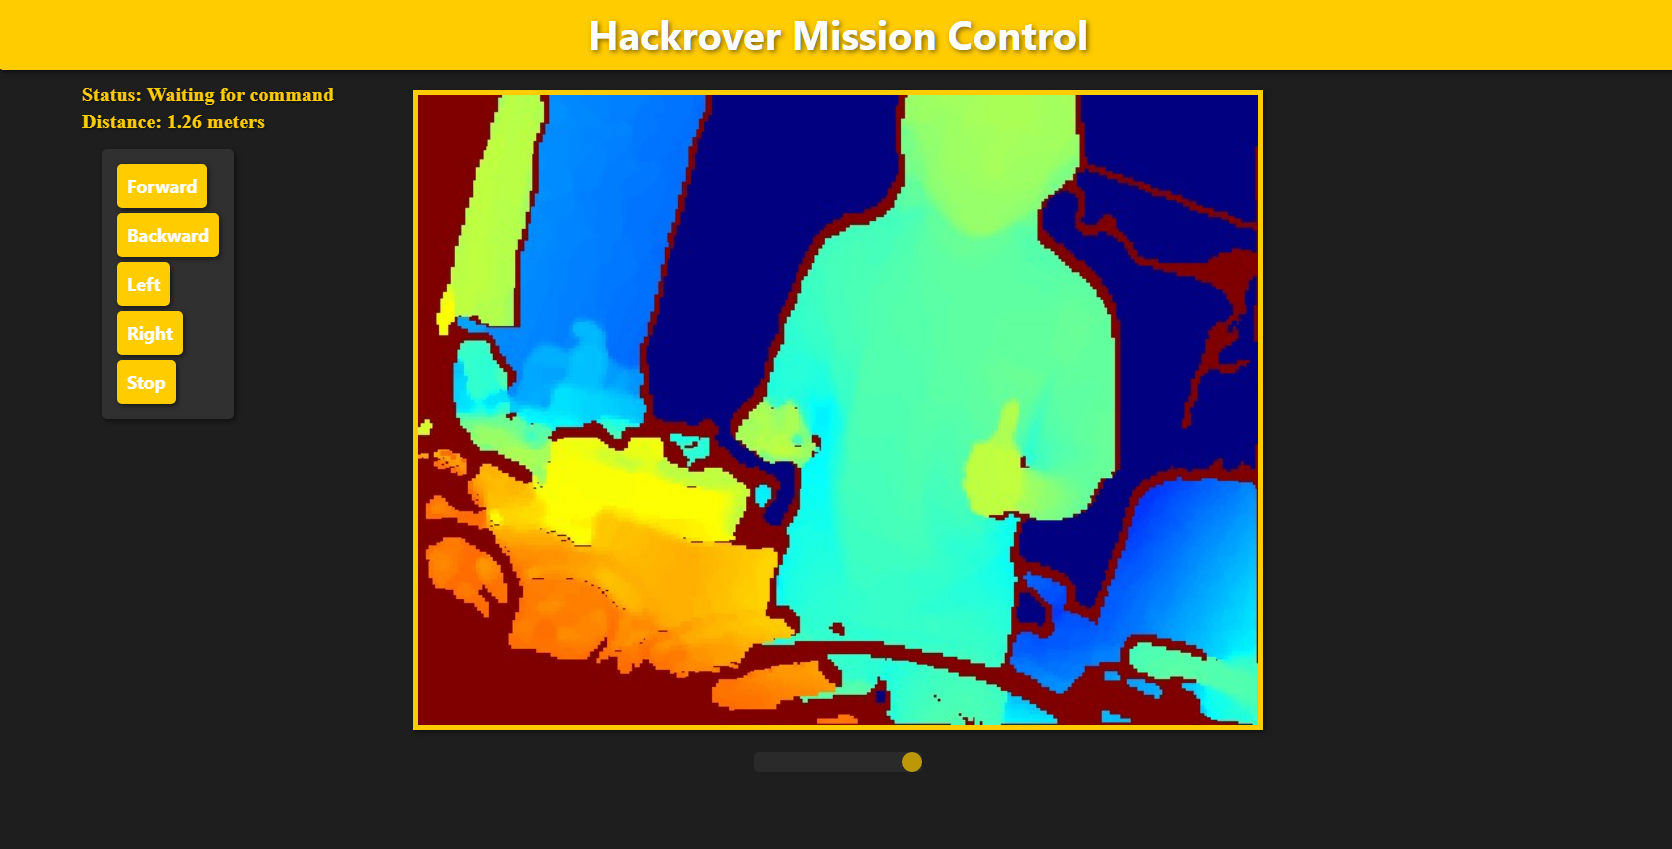
\includegraphics[scale=0.25]{Photos/hackrover mission control}

	\subsection{Best Use Practices Report}
	There are virtually no `Best Use Practices' for any mechanical or electrical subsystems of our rover. We designed with the intent of offloading physical configuration from the user; all best use falls in the lap of human-computer interaction, and our computer engineers.
	
	Minimum best-use expectations are relying on custom designed launch scripts for initial setup. We want the user to avoid typing into any terminal, or plugging directly into the rover with computer. This decision acts to simplify the setup process, and also hide information. Hiding information is important because it removes the opportunity for making careless mistakes. 
	
	Once the launch scripts - activated with simple turn on or button press - setup the rover, the user should spend all their time within the command center GUI, and the controller in their hands.

	\subsection{Usability Requirements Document}
	The first product will be a robust rover system with a modular, programmable software architecture created in ROS and hosted on the central Xavier or Nano computer. Booting the rover system will be straightforward, and all background tasks for effective startup will be offloaded from the user via automation by simple scripts. The user will be able to easily control the rover from one of many control paradigms, and see useful output on a monitor through a custom designed GUI. 
	
The form factor of the rover itself will be akin to last year: a PCB interfacing the Xavier/Jetson with an RBPi and motors; and a LiDAR and communication stack communicating with the Xavier/Jetson. All UI will be handled through ROS. 

\pagebreak
	
\section{Requirement Documentation}
	\subsection{Decisions and Rationale}
	The final plans for the build phase will - at a minimum - include the creation of one first iteration puzzle panel, and one first iteration disaster rover (Mimir). Experiencing success with these sooner than later will prompt us to improve upon the base design with further iterations (which introduce more electronics, better mechanical housing, cleaner code), as well as create more puzzle panels and competition rovers.
	
		\subsubsection*{Puzzle Panels}
		The goal of the club, competition, and these puzzle panels was to serve as a pedagogical tool for interdisciplinary engineering for UW students. To that end we researched game design and player learning. The most wealthy source was Portal and Portal 2, which - like our puzzle panels - see modular puzzles composed of smaller puzzle elements. Within the game you can enter a `developer' mode, causing small interactive speech bubbles to appear throughout the map; selecting these bubbles plays back the developer's log. The most important log discussed the importants of iconic puzzle elements with increasing complexity of interaction, starting from the most foundational operations. For example, the player's first puzzle is to place a large box onto a bright red button that opens a door; the next puzzle sees two boxes and two buttons. Obviously progression doesn't need to be that dull, but the concept stands.
		
		--------INCLUDE IMAGES OF PORTAL WITH SPEECH BUBBLES
		
		From this we decided the puzzles - for which there would be four, one to each floor - must increase in difficulty. Each puzzle, being comprised of the same fundamental elements, must use these elements in ways of increasing complexity. The fundamental elements must be easily understandable with minimal interaction. We decided upon 6-7 different elements, including ultrasound sensors, push-buttons, and potentiometers.
		
		Modularizing our elements was important for their manufacture and control methods. With modular components we can off-the-shelf Arduino-compatible actuators and sensors, and build icon housing around them. This should also make creating software in OOP environments easier. 		
		
		\subsubsection*{Rover}
		The rover will operate in earthquake, warzone, and building collapse environments. it needs to be rubble resistant, have a low center of gravity, and stocky. The electrical systems that power it must be reliable, robust, and deliver clean energy. The software framework that underpins it must be modular for future development or rapid on-site changes. This modular software framework will also translate into the physical of the rover design, with mountings and electronic connections that are modular.
		
		The rover also sees the addition of a novel, camera control method the form of a Stewart platform. Traditionally the Stewart platform has been a parallel robot with 6 linear actuators. The significance is that this device can move in 6 DOF, and reverse kinematics can be used to calculate actuator position - simply plug in desired position and a math model determines actuator output. Recently roboticists have been popularizing a Stewart platform that uses rotational servos - as opposed to linear actuators - and the designs/models are promising, especially for their cost effectiveness. We plan on a Stewart platform controlling the LiDAR camera.

	\subsection{Tier 1 Schematics}
		\subsubsection{Mechanical Team}
		An early mapping of the rover seen in THE FIGUREEEEE reflects what we actually intend to build. As you can see, the chassis is divided into drive base and housing, where housing is further subdivided into tiers. The size of components mostly dictates the function/organization of tiers; but, conveniently electronics and microcontrol will occur in the bottom tier, higher level microcomputer control and networking will occur in the second layer, and sensing with the LiDAR will occur at the highest layer.
		
		-----NEEDS IMAGE OF LAYERS
		
		\subsubsection{Electrical Team}
		The puzzle panel will be powered by a power source (wall wart) that will connect to a power distribution system (PDS) which will power the actual puzzle panel game. The PDS itself will be able to power each and every hardware with enough power.

		The rover will need a power source that can provide enough reliable and disturbance-free power to all hardware. A power distribution system will be needed to safely distribute enough power to each hardware and also, size of the PDS will be dependent on what the final size of the mechanical system will provide for the PDS to fit in.  
		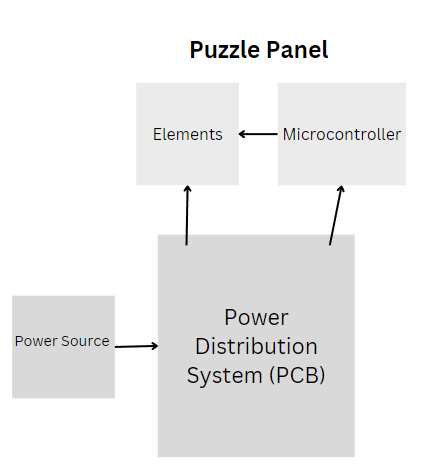
\includegraphics[scale=0.8]{Photos/Puzzle Panel tier 1 schematic}
		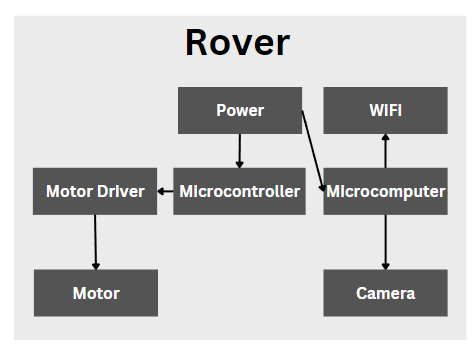
\includegraphics[scale=0.8]{Photos/Rover tier 1 schematic}

	\subsection{Tier 2 Schematics}
		\subsubsection{Mechanical Team}
		Provided thanks to retrospect, we can see a better visual of component placement in Fusion360. Here the same tiered `territories' exist within the rover design. Components included in the image should give some idea of function.
		
		--------NEED DRIVE TRAIN
		--------NEED BASE LEVEL
		-----NEED MIDDLE LEVEL
		------NEED TOP LEVEL
	
		\subsubsection{Electrical Team}
		The puzzle panel schematic that is shown details the connection of power for the puzzle panels. The connection starts from the power source which is a wall wart that we will use to power the puzzle panel. The wall wart would output its maximum voltage to the power distribution system (PDS) which then will be distributed to every electrical component. The PDS is constructed to be able to provide different ranges of voltage to meet the power requirements for any electronic component. The puzzle panel itself will be operated by Arduino or PCBs which control the function of the puzzle panel through its connection to the electrical components. Each puzzle panel differs by its own use of electrical components and by the function of its Arduino. 
	
		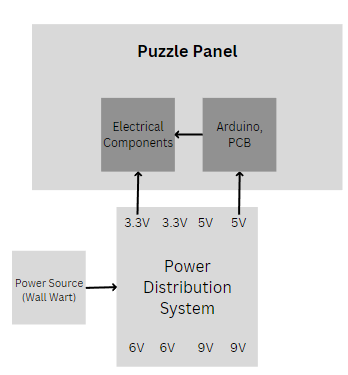
\includegraphics[scale=0.8]{Photos/Puzzle panel simplified}
		
		The simplified Rover Electrical Schematic details the connection from the power source to the rest of the electrical components that are present in the system. The hardware involved are essential for controlling the rover. The Jetson Nano is a microcomputer that runs multiple neuron networks, meaning it can handle multiple tasks at the same time. A Wifi component is built into the Nano which can be controlled wireless without having to control with a physical wire connection. The Arduino Mega is a microcontroller that has the built in code which sends control signals to the motor controllers. The Nano is commanded by the user which the user would send a command to the Nano, and depending on the command which will be sent to the Arduino Mega. This scenario is when both the Nano and the Mega talk to each other with the Nano being controlled by the user have the final say. This relationship works the same way with the Arduino in the stewart platform. The signals that are going to be sent to the motor controllers in the motor system, contain directional/control signals. The motor controllers act like a mini-computer which receives the signals from the Arduino and transmits those signals to the motors which as a result, runs the motors. The arduino with the stewart platform carries the LiDAR camera which monitors live footage and sends back the information in a wireless connection back to the user. The stewart platform is formed with many small stepper motors that reorients the position of the platform from the arduino signals.  
		
		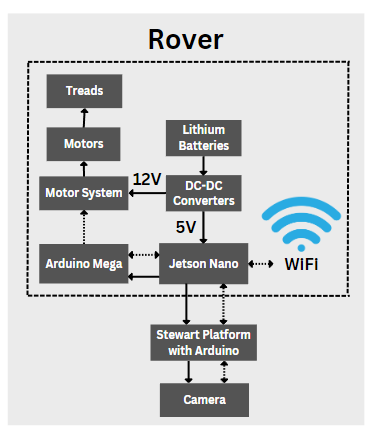
\includegraphics[scale=0.8]{Photos/Rover schematic simplified}
	
		\subsubsection{Software Team}

		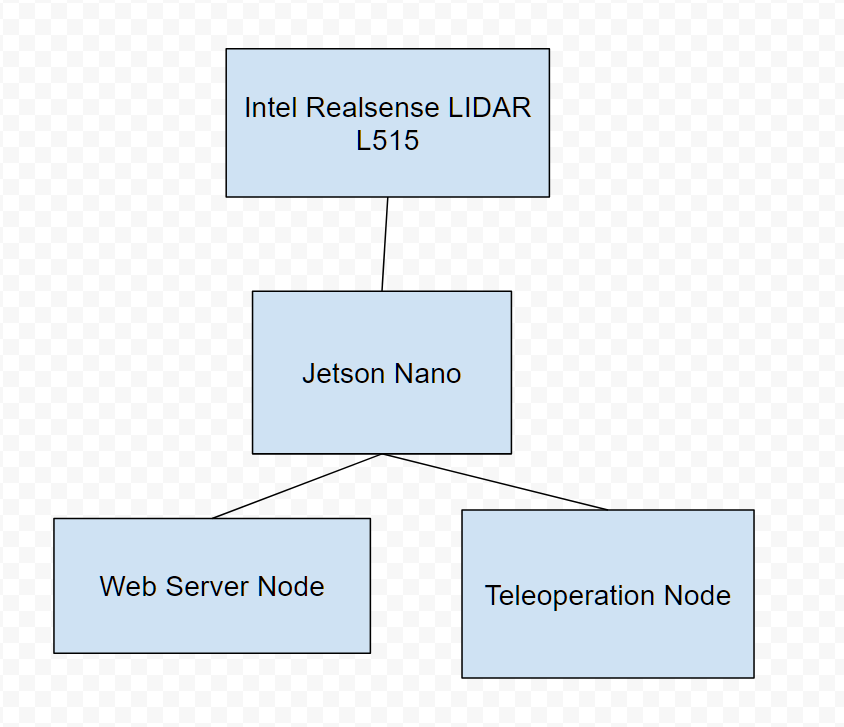
\includegraphics[scale=0.3]{Photos/LIDAR nodes}

		The FIGURE details the interaction between the Intel RealSense LIDAR L515 with the NVIDIA Xavier. The ROS node that is used as the publisher of the LIDAR image data to then be sent to a subscriber to the image data uses image\_ transport as the library to export the images from the LIDAR to the processing node in a low-bandwidth compressed format to reduce latency. The image processing node has computer vision models within the node to process the image using OpenCV, which is then sent to the Xavier as data that the Xavier will use for further motion logic or displaying the image to the user.

		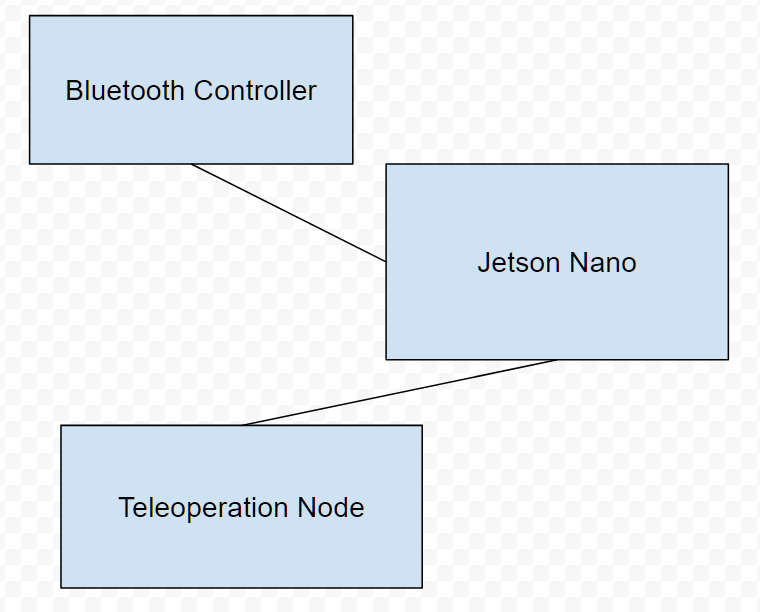
\includegraphics[scale=0.3]{Photos/controller node} Controller System Design Diagram:

		The FIGURE details the interaction between controllers (Xbox, Playstation, etc type controllers) with the NVIDIA Xavier. There is the package that contains the motion logic that the previously mentioned LIDAR interacts with to send motion controls to the Xavier as well as a ROS node that takes controller inputs and processes them to be sent to the motion logic package. The data going from the controller to the ROS controller is analog data that Linux can already understand and there are pre-existing ROS libraries to use controllers. The controller node itself will send out motion commands to the motion logic package which will then send motion data to the Xavier. We also want to ensure that the controller node itself won't do any illegal inputs so we want to create a connection between the motion logic package and the controller node in case of inputs that were not friendly to the rovers motion.	
	
	\subsection{Tier 3 Schematics}
		\subsubsection{Electrical Team}
		The PCB of the puzzle panel will start with a wall wart which would output a specified amount of voltage to the PDS. The PDS will be made up of three levels, each level containing rows of buck modules that are placed in parallel and their function is to step-down the input voltage from the wall wart, down to the amount that is needed for an electrical component. Each buck module will distribute different amounts of voltage due to each electrical component within the actual puzzle panel, requiring different levels of voltage.
		
		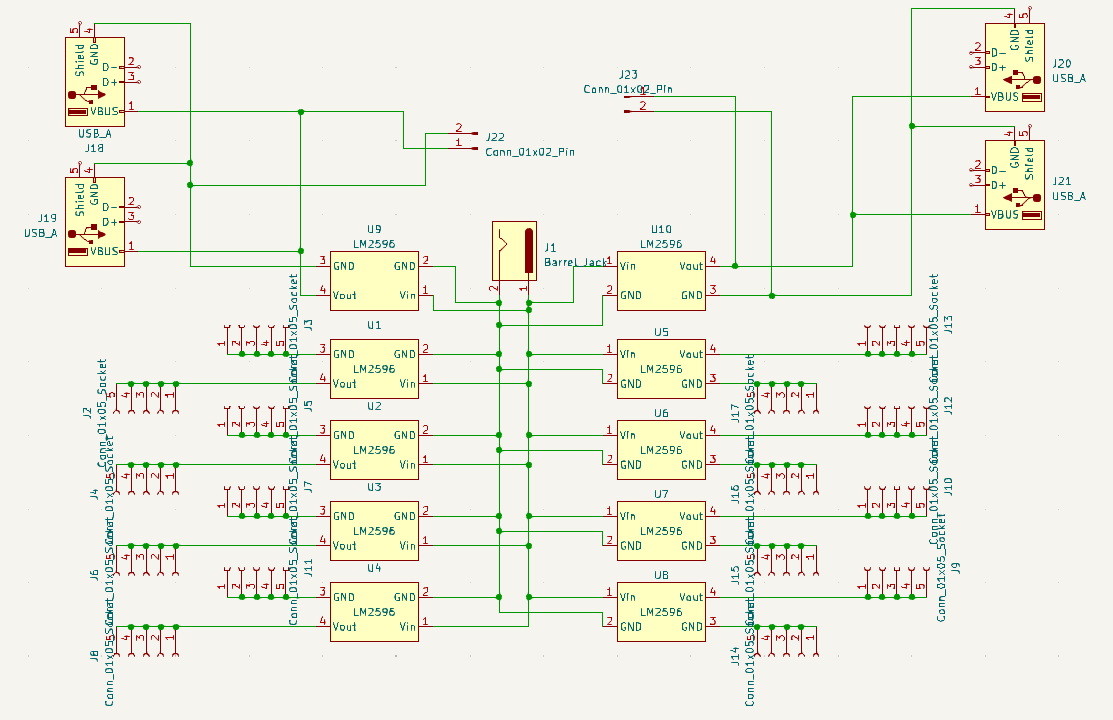
\includegraphics[scale=0.7]{Photos/Puzzle Panel schematic 1}	

		The rover will be powered by lithium batteries that can provide enough voltage or power to the whole rover. The 12V DC-DC buck converters which outputs a set amount of voltage of 12V in which the motor controllers are directly powered by. The small buck converters, convert the 12V to 5V which powers the Jetson Nano, Arduino Mega, Stewart platform, and et cetera, which are necessary in the system to control both the distribution of power. 
		
		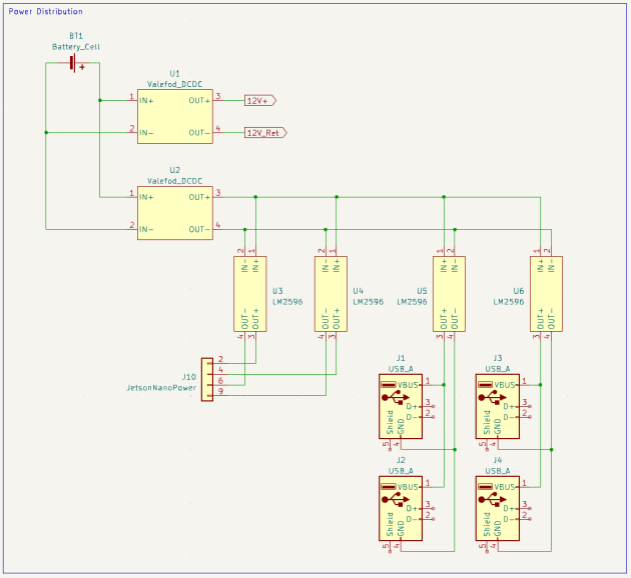
\includegraphics[scale=1.05]{Photos/Rover schematic 1}

		The power will be distributed with buck modules to power each component at its needed level. And the step-downed power will then be delivered to the Arduino Mega, Jetson Nano, Motor controllers, and other components which will run the whole rover. This PCB is constructed to use four motor controllers but in this project, two are used to operate the rover. The four USB ports output 5V which are used to provide power to any additional add-ons to the rover, which means different hardware can be added. 
		
		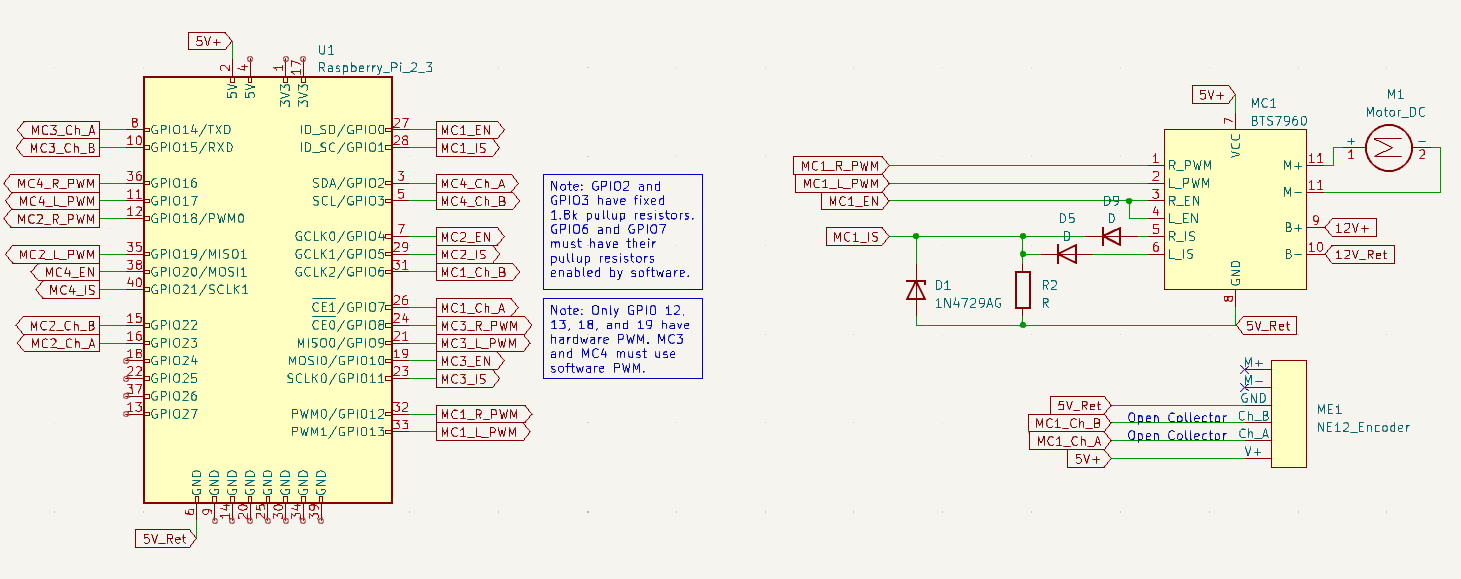
\includegraphics[scale=0.95]{Photos/Rover schematic 2}	
		
		Other miscellaneous elements or components like transistors, diodes, resistors are essential in keeping the digital signals at safe levels, to prevent current/voltage spikes.
		

		\subsubsection{Software/Computer Team}
	Starting with the LIDAR integration the main connection is between the publisher and subscriber node of the LIDAR image. The publisher node will be outputting a compressed formatted image to the subscriber through the image\_ transport API. Within the processing node (subscriber to the image data) we can use OpenCV to translate the image that is being collected from the publisher to be created into a model that the rover can use to identify what is being shown in the image. This can be done with a point-cloud model and computer vision techniques. After the image is processed, the image itself is sent to the Xavier to display to the user and the image data with motion commands is sent to the motion logic, where the motion logic will then determine whether the images motion data is relevant to motion objectives. The latter is a back and forth process between the subscriber processing node and the motion logic component. 
The second part with Xavier for this capstone project is the controller node. The main connection will be between the controller node that takes in controller information and the motion logic. This will also be a back and forth process between the two since the motion logic may not want to perform the actions that the user is inputting into the controller. 

	\subsection{Estimation of Cost of Goods}
	The final estimation of cost falls around 1,500 dollars. Overtime, the cost changes due to the major design decisions have to be made by electrical and mechanical leads before a final order can be placed. An each orders are done on a weekly basis with each section having a total shown below. 
	
	The estimate costs of goods of the Electrical components falls to 915 dollars which includes miscellaneous components that are already in our inventory that costs around 400 dollars. The Mechanical components falls to 233.24 dollars """(include also, estimation costs of miscellaneous mechanical parts already in inventory)"""

	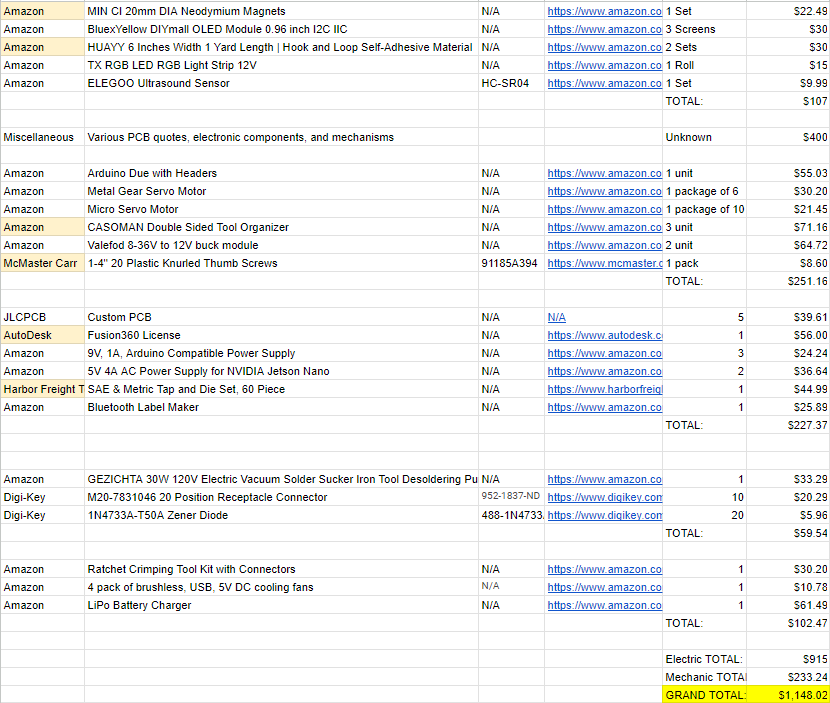
\includegraphics[scale=0.9]{Photos/Bills of Material}

	\subsection{Schedule}
	We make use of an online, free, Gantt software accessible to anyone. A screenshot of only a portion of our schedule can be seen below. Our project is split into mechanical, electrical, and computer sections, each with 'sub-projects' which have their own schedule proscribed with dates, information, background, etc.

	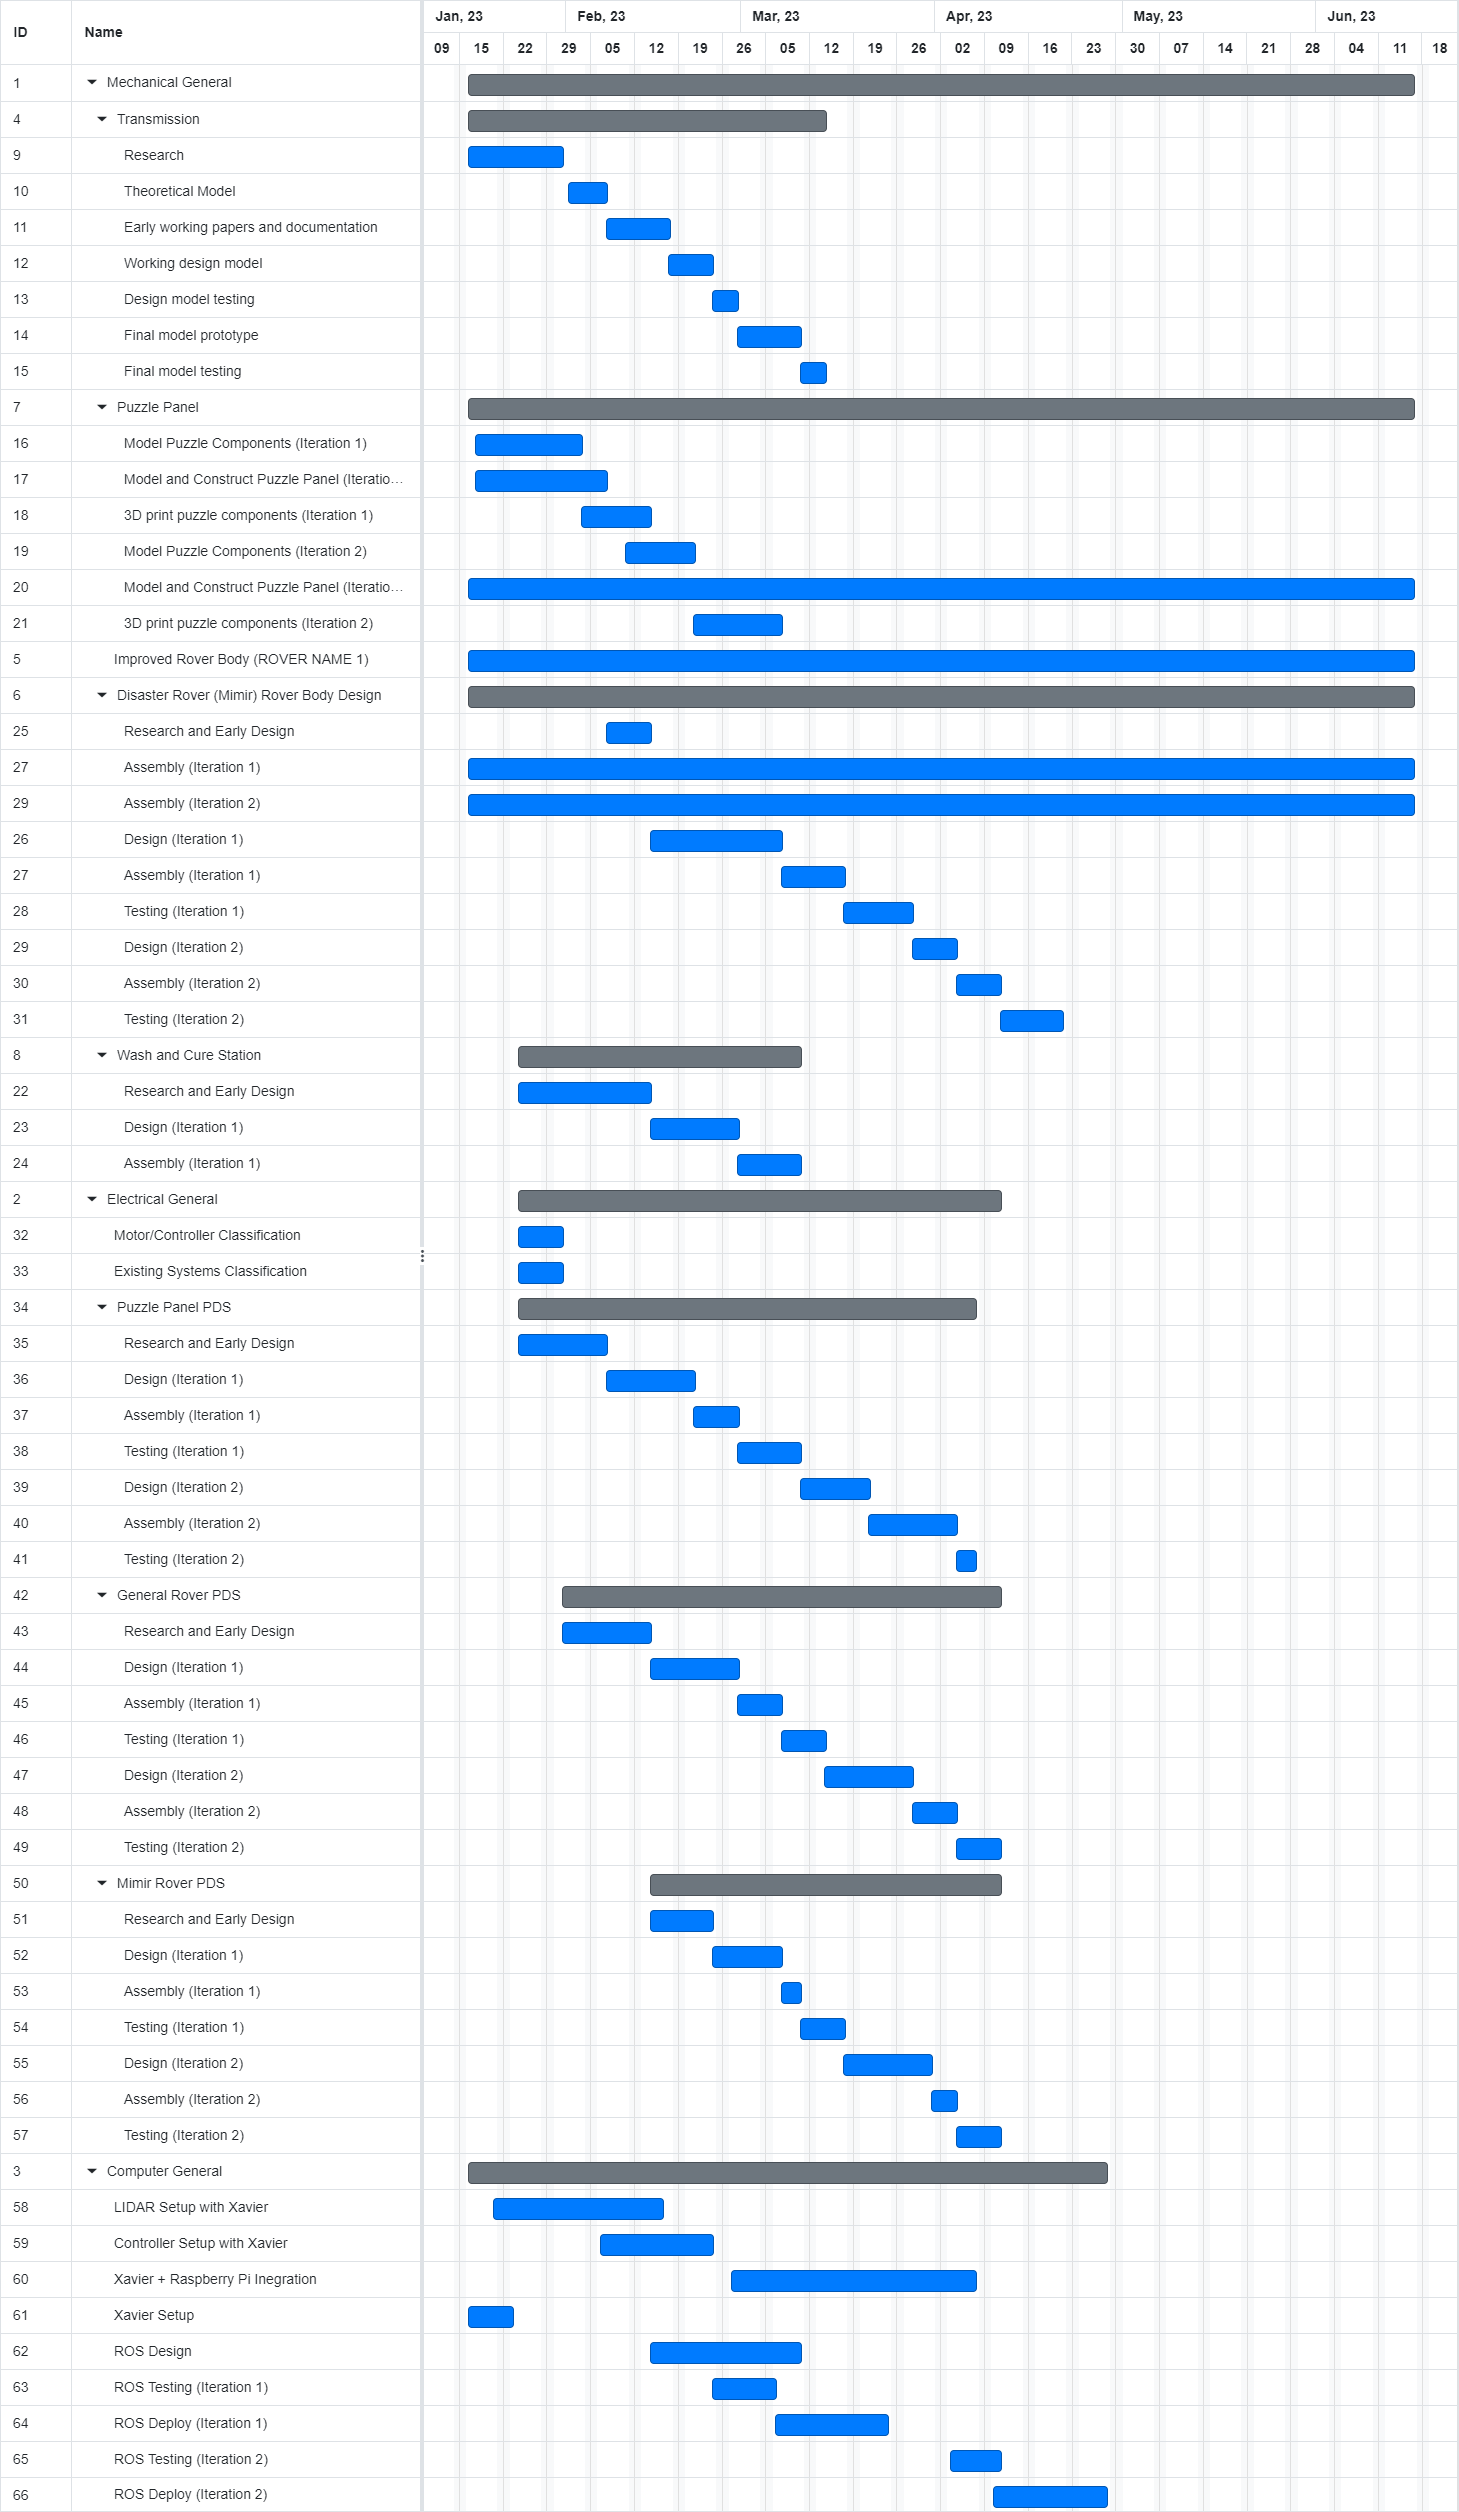
\includegraphics[scale=0.3]{Photos/Gantt Chart}

\pagebreak	

\section{Concept Development}
	\subsection{Technology Mapping, Risk Analysis, and Feasibility}
	The minimum product we'll create is a disaster rover, for which we have all the needed components. Functionality will be ensured with the software created to operate well-planned electromechanical systems. Usability will be ensured with effective documentation and simple controls. A well ordered rover with ease of control and robust build will be necessary and capable for further business; though, our client is the UW, so we have little concern for how this would  sell.
	
	The disaster rover would need to traverse rugged terrain. A compact frame with a well-set center of gravity and tank treads would allow it to path in any environment. Falls or tumbles would be mitigated by a 'domed' upper chassis that ensures it always lands on its base. Operators will be able to connect to it easily and wirelessly, (ideally through browser), and control with easy to understand, video-game based control schemes. All electromechanical systems would interface through robot operating system (ROS) housed on a central, Xavier computer. Focusing on electrical and mechanical systems independently: electronics will convey clean, modular power to various components through LIPO batteries. Clean and modular, I stress again, are the focus; devices like the Xavier have stringent voltage and current regulations. Modularity is desired, as future iterations will see different parts added or subtracted; ideally the only aspects affected here are battery life. Everything is contained on a central PCB, improving physical efficiency further. The mechanical systems need to be robust and sourceable. Through the use of aluminum frame, higher end FDM and resin plastics, and (hopefully) casting, we'll be able to create a protective housing for all electrical and computer components. Motors will be mounted directly to the frame with little (or no) geared transmission, depending on the speed and torque output of what motors exist. A small frame is preferred to minimize stresses. Further research into the mechanical engineering of motion mechanisms is needed before a better description can be provided. 
	
	The greatest risks are addressed in order: computer, electrical, mechanical. The computer model only addresses the function of interdependent components in extremely ideal conditions. A disaster environment won't be perfect, and the rover needs to get itself out of sticky situations if communication is lost or electromechanical systems aren't behaving perfectly. The electrical system could fail to provide stable enough current or voltage, or locales of high power draw could result in heating that leads to failure. It's possible the arrangement of components doesn't permit a long enough battery, or results in excess inefficiencies. The mechanical systems may fail about shafts or joints, and the production of gears (as they'll be printed) may be outside of tolerance.
	
	To address the stated risks we need effective testing and redundant systems. Computer models need to simulate circumstances where power delivery or mechanical failure causes issues. Further, boot scripts and backup communication protocols need to exist. Electrical systems have to be tested under every conceivable driven condition, with a focus on clean power. Mechanical systems need to be simulated, constructed with high factors of safety, and modeled physically with test rigs.
 	
 	\subsection{Component Technology Research}
 	\textbf{Puzzle Panel}
 	The competition puzzle panels are the only physical manifestation of the competition. They will address mechanical, electrical, and software modularity. To these ends, small electromechanical puzzle components will be designed; arranged properly they will constitute a puzzle panel. The components will be Arduino compatible, have iconic housings for easy robot interaction and future AI solving, and attach to the puzzle panel physically via velcro. The physical puzzle panel will be clad in velcro. 
 	
 	To achieve electrical modularity, a custom PDS which delivers clean voltage of choice will be designed. A wall wart provides power to the PDS, which distributes it to adjustable, low voltage buck modules. The entire PDS will be housed and mounted to the back of the puzzle panel, another task of the mechanical engineer. Students will be able to plug their electromechanical puzzle elements and Arduino into the PDS and be confident the power they recieve is reliable and free of disturbances.
 	
 	To achieve software modularity, custom software libraries written in the Arduino language will be created. Students can drag and drop into their control programs, and access custom functions. This will not only drastically simplify control programming, but also improve prototyping.
 	
 	\textbf{Rover}
 	To address environmental constraints imposed by the context of disaster relief, our rover will have a rubble-resistant chassis design, and encased, centralized electrical PDS. We will also try to achieve modularity mechanically, electrically, and software wise. To achieve mechanical modularity, the drivetrain will be constructed of stock aluminum parts, and the housing will see a tiered system with adjustable mounting and plenty of open space. In addition to these two major rover aspects, we will have a rotational servo actuated Stewart platform that controls our LiDAR camera; all other components on it will be 3D printed.
 	
 	To achieve electrical modularity the battery connector will be common, connecting into two buck converters. These buck converters are responsible for stepping down voltage to power logical (5V) and power components (12V). The unique property here is any battery with the same connector may be used. The PCB we designed itself is the PDS, providing power to all logical and actuative components. On the PCB we will add extra ports and adjustable buck modules for unanticipated, future modifications, or alternative designs. Though our rover Mimir only uses two motor controllers, the PCB will be designed with four so it may be repurposed for other designs.
 	
 	To achieve software modularity we will be developing our architecture in ROS. Each component, interaction, data processing procedure, etc can be respresented as a modular `node' that can be added or removed from the final build and launch script.
 		
 		\subsubsection{EE Circuit Models}
 		-------------NEED TO COME BACK TO THIS
 		
 		\subsubsection*{Stewart Platform}
 		The Stewart platform houses and controls the motion of the LiDAR. Early designs of the electronics are presented below. The first iteration we created was simply proof of concept, and to prototype the control software. It used a GikFun solderable breadboard as the base for our power electronics and signal electronics, and all components. An early mockup of the electrical schematics can be seen in figure -----INSERT REFERENCE HERE, and the physical, manufacture control board can be seen in figure ------INSERT REFERENCE HERE. We do have plans to have the control board be professionally printed, or seek out a third party servo controller, if possible.
 		
 		----INSERT IMAGE OF ELECTRICAL SCHEMATICS
 		----INSERT IMAGE OF FINAL BOARD
 		
 		The Stewart platform was controlled by an Arduino Due. The Due is effectively a beefier version of the Arduino Mega: it has the same footprint but faster processing speed and bigger memory. The math model-based script we're using to forward angle inputs to Stewart platform actuation is extremely intricate and process intensive. A visual of the Due can be see in figure -----INSERT REFERENCE HERE
 		
 		-----INSERT IMAGE OF DUE
 
 		\subsubsection{Mechanical Models}
 		Mechanical modelling was completed incrementally and with lots of thought on a day by day basis. Plenty of notes were taken, and it would be a waste to ignore them. That being said, content must be streamlined in the MegaDoc presentation. I present various moodels throughout all the stages.
 		\subsubsection*{Puzzle Panel}
		The puzzle panel can be divided into the panel itself and the small components that constitute it. The design rational was mentioned above, so I won't repeat myself. In figure ----INSERT REFERENCE is the Fusion360 model of the puzzle panel completed; one instance of the panel was constructed in real life, a photo of it seen in figure -----INSERT REFERENCE.
		
		-----INSERT IMAGE OF PUZZLE PANEL IN FUSION360
		
		-----INSERT  IMAGE OF REAAL LIFE PUZZLE PANEL
		
		There were a small collection of electromechanical puzzle components that made the cut: (1) button, (2) servo motor, (3) ultrasound sensor, (4) light strip, (5) potentiometer, and (6) wall. The specifics of each and every one isn't particularly important, but what is noteworthy is the manufacturing procedure. Each component selected is Arduino-compatible, purchased in bulk from the internet. A custom, 3D-printed housing is created and then encases the part, enabling it to be attached to the board for student  use. In figure ----INSERT REFERENCE is just one example of these components, an ultrasound sensor, modelled in Fusion360, if you inspect the puzzle panel in the previous section, you might notice its use.
		
		-----INSERT IMAGE OF ULTRASOUND
 		
 		\subsubsection*{Rover}
		The rover can be split into its drive base and component housing. Seen in figure ----INSERT REFERENCE is the drivebase without treads, assembled in Fusion360. The drivebase was adopted from the previous year's design, so details of component selection arren't extremely relevant here. Motor were changed, however, as analysis of performance revealed last year's team made poor selection resulting in low efficiency; this analysis is elaborated upon in the methodology section. We swapped out the 612RPM motors for 118RPM motors, seen in figure ------INSERT REFERENCEE; you might believe the speed would drastically decrease, but the 612RPM motors were being run at such poor performance they were already 1/12th their quoted maximum. The 118RPM motors were significantly more efficient and roughly the same speed.
		
		-----IMAGE OF DRIVEBASE GOES HERE
		
		-----IMAGE OF MOTORS GOES HERE
		
		The component housing was design per our specifications and mention before. We have three tiers: bottom, middle, and upper. The bottom tier houses the PDS, and microcontrollers for the motors and Stewart platform; see this tier in figure ---INSERT  REFERENCE. The middle tier houses the Jetson Nano - the master microcomputer running ROS - and the 3-in-1 networking device; see this tier in figure ----INSERT REFERENCE. The top tier houses the Stewart platform, it being discussed in a later section; see this tier in figure -----INSERT REFERENCE.
		
		----IMAGE OF EACH TIER FROM FUSION360
 		
 		\subsubsection*{Stewart Platform}
 		The Stewart platform houses and controls the motion of the LiDAR. We're using the same LiDAR as years prior, so we don't feel the need to discuss it in detail or present images; it's a Intel RealSense LiDAR L515. Early designs of the Stewart Platform are presented below. The first iteration we created was simply proof of concept, and to prototype the control software.
 		
 		\begin{figure} [h]
			\centering
			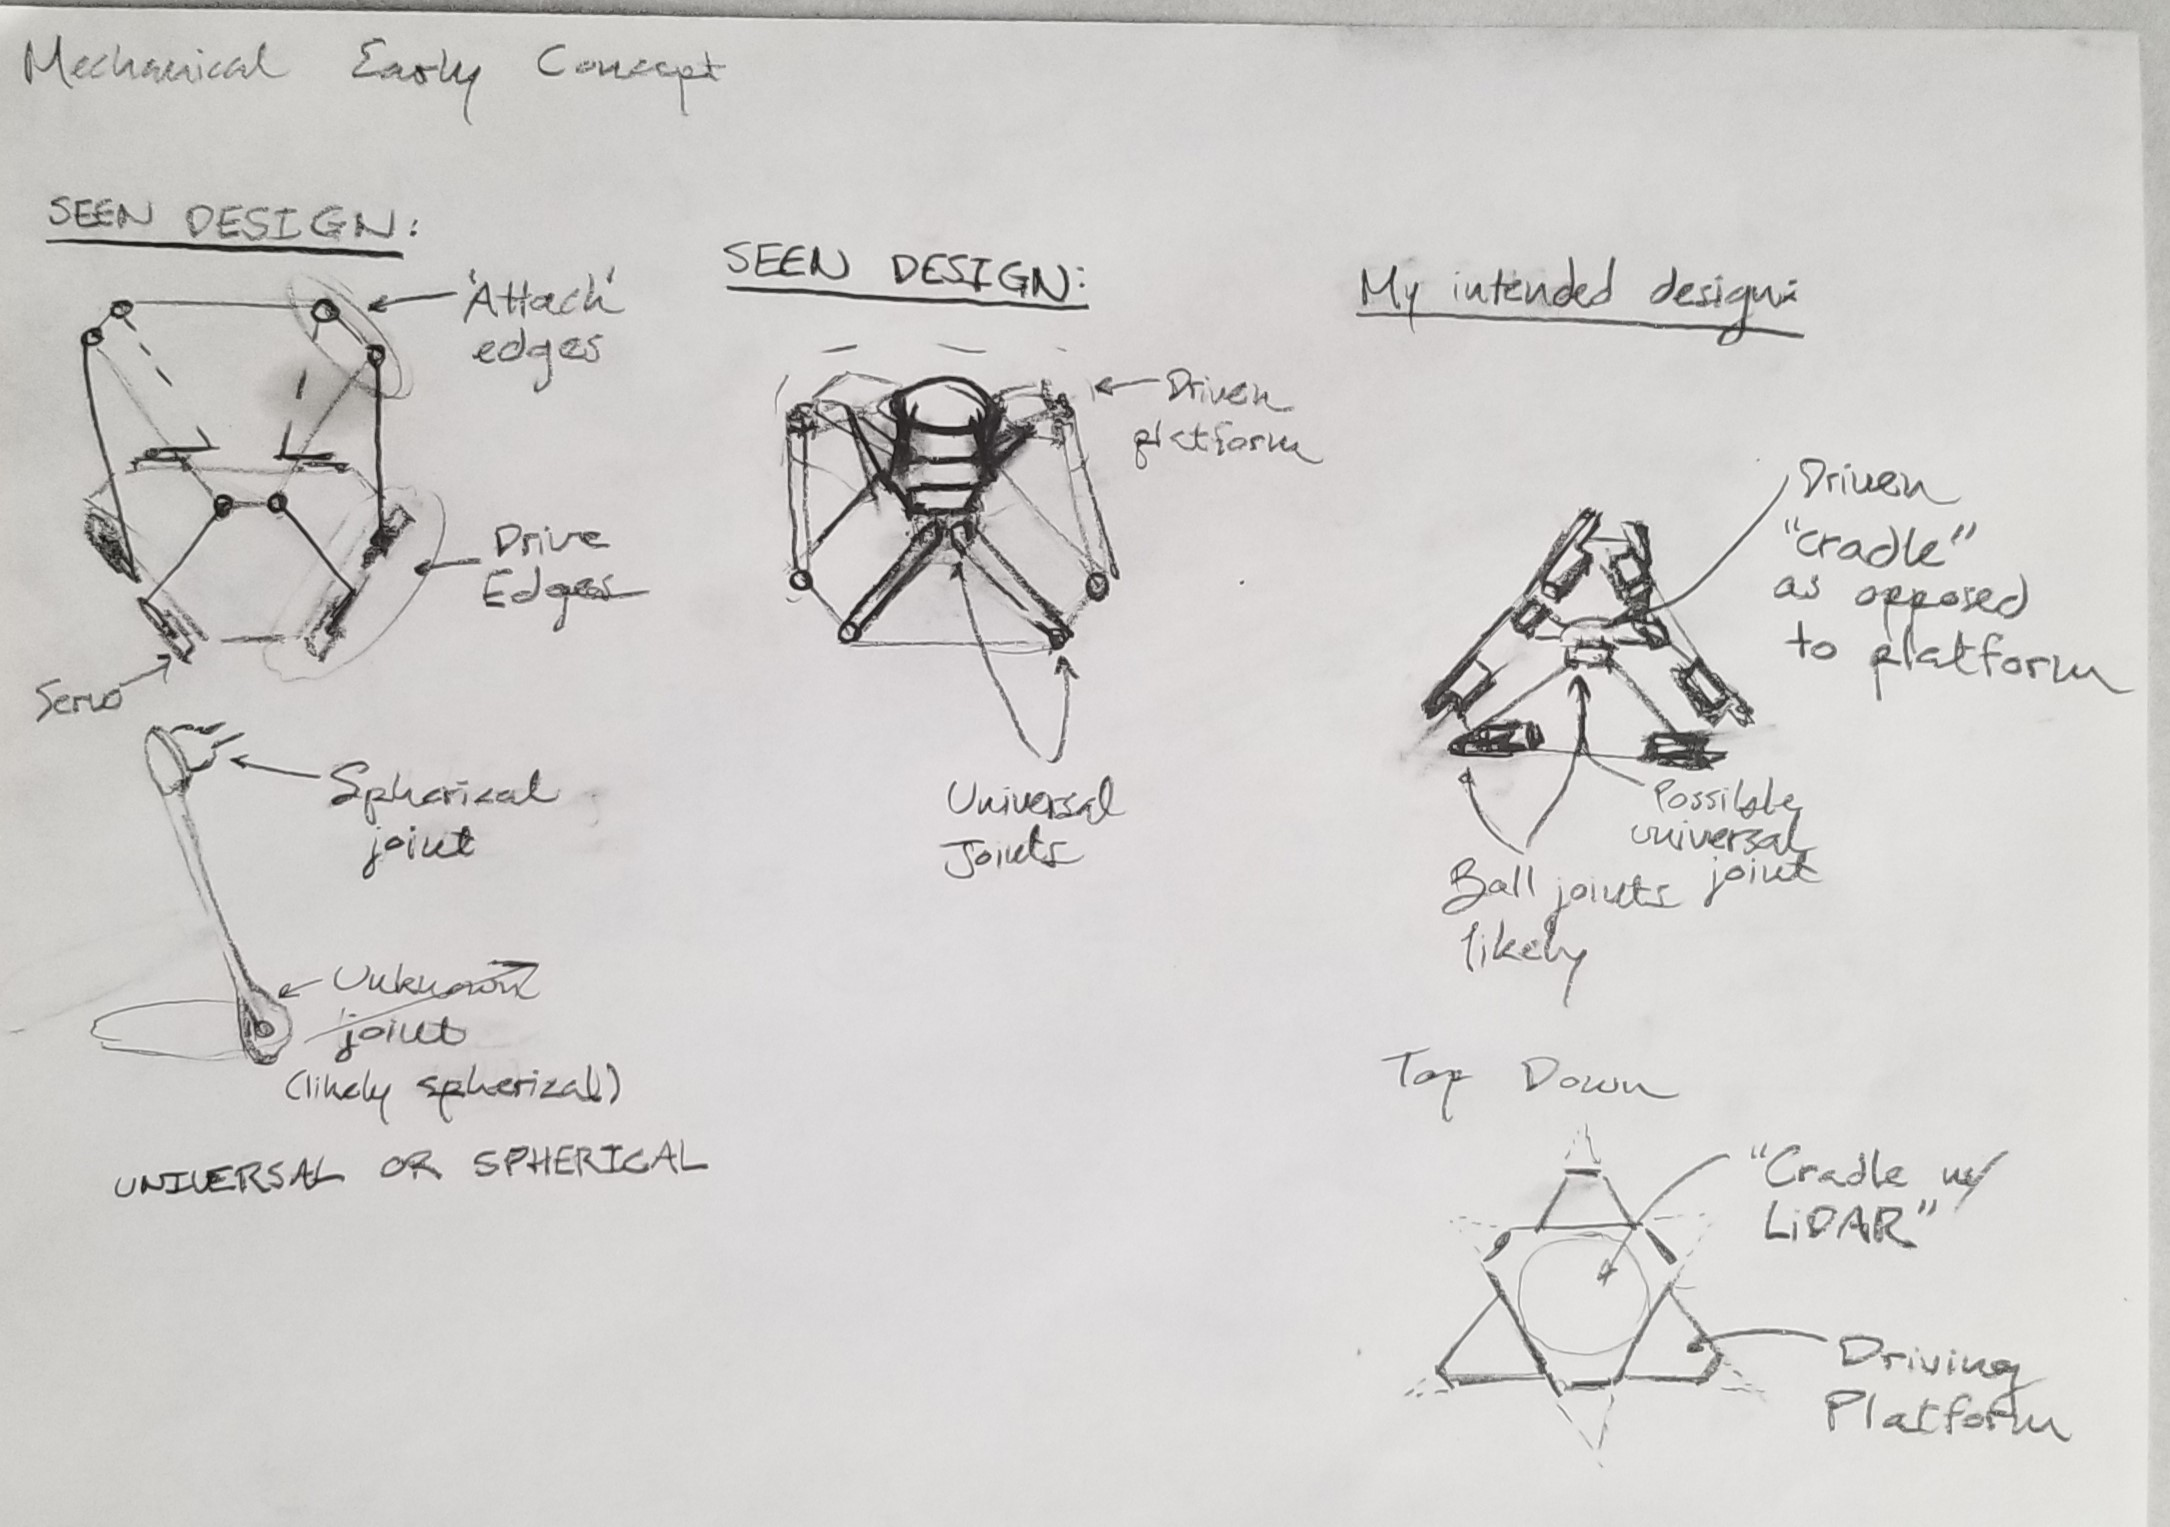
\includegraphics[scale=0.2]{Photos/early_mechanical}
			\caption{Mechanical sketches seen at the right}
			\label{basic_mechanical}
		\end{figure}
		
		Early on I decided to print the housing, linkages and ball joints. Most parts were custom designed, but some were 3D models that were sourced from McMasterCarr, then modified, as seen in Figure \ref{ball_joint}. The printing was completed on both resin and FDM printers.
		
		\begin{figure*}[h]
			\centering
			\begin{subfigure}[h]{0.34\textwidth}
				\centering
				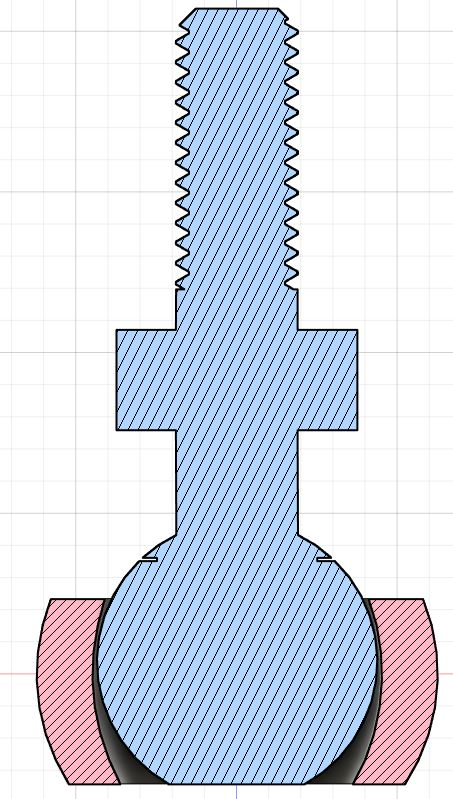
\includegraphics[width=\textwidth]{Photos/section_ball_joint}
			\end{subfigure}
			\hfill
			\begin{subfigure}[h]{0.65\textwidth}
				\centering
				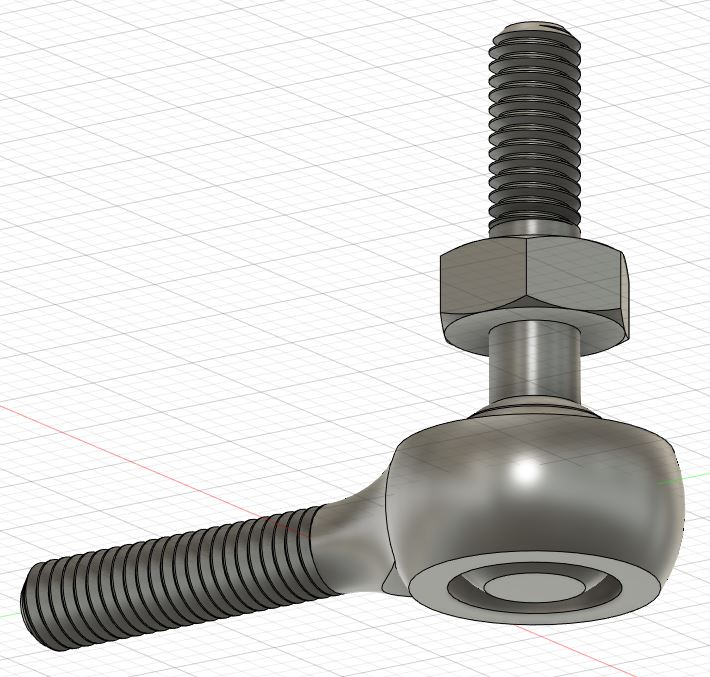
\includegraphics[width=\textwidth]{Photos/ball_joint}
			\end{subfigure}
			\centering
			\caption{Section of the ball joint showing no interference, next to its 3D model}
			\label{ball_joint}
		\end{figure*}
		
		A final first iteration can be seen in figure \ref{final_assembly}. It includes and top and side view. This version worked out well for prototyping, but wasn't our final.
		
		\begin{figure*}[h]
			\centering
			\begin{subfigure}[h]{0.34\textwidth}
				\centering
				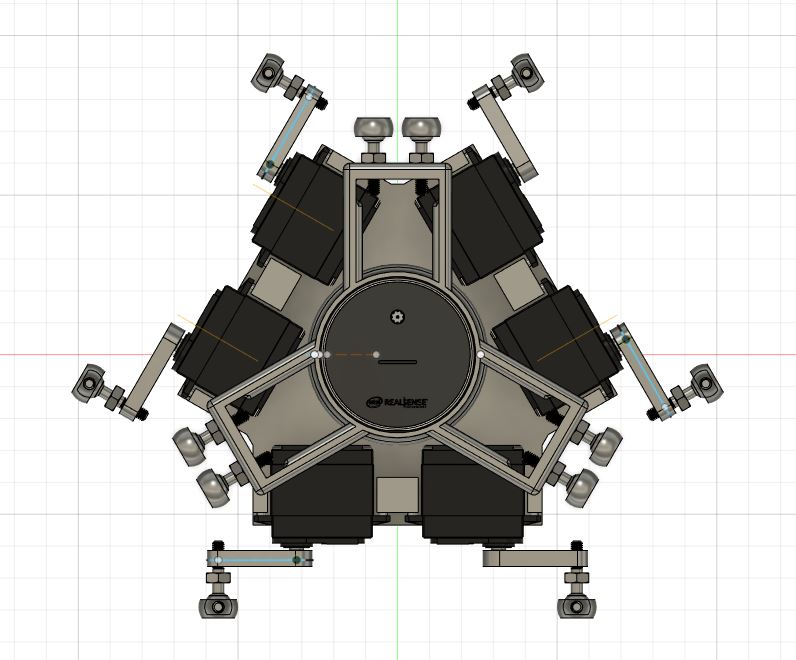
\includegraphics[width=\textwidth]{Photos/assembly_top_down}
			\end{subfigure}
			\hfill
			\begin{subfigure}[h]{0.65\textwidth}
				\centering
				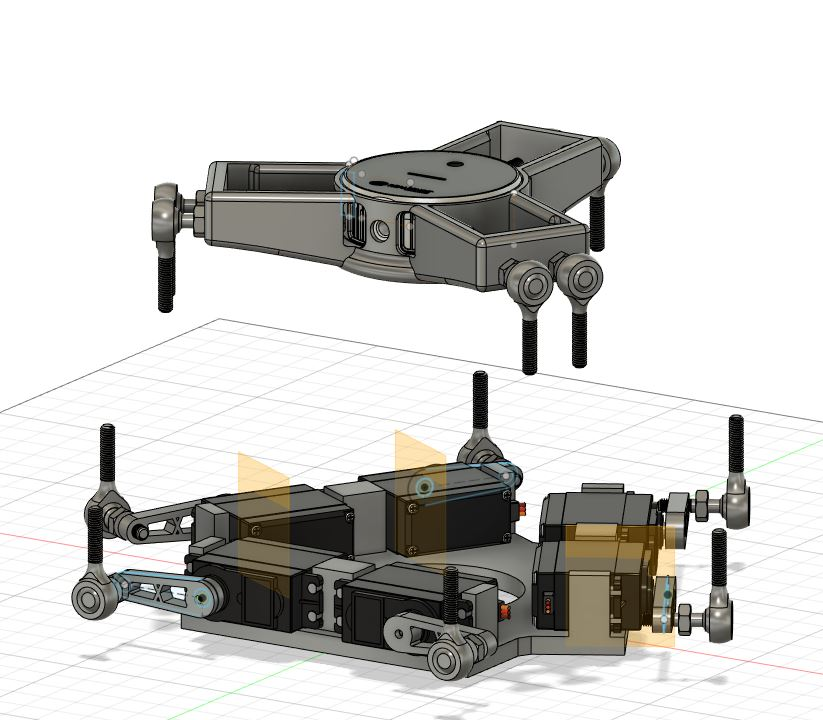
\includegraphics[width=\textwidth]{Photos/complete_assembly}
			\end{subfigure}
			\centering
			\caption{The final first iteration assembly}
			\label{final_assembly}
		\end{figure*}
 		
 		In the second iteration we made sure the platform mounted to the rover. We also improved the structure by making the ball joints and linkages permanently connected and printed with a stronger resin. A housing for the LiDAR was created on an FDM printer. The final version can be seen in figure ----INSERT REFERENCE.
 		
 		------FUSION360 IMAGE OF STEWART PLATFORM
 		
		\subsubsection*{Risk Identification}
		Risk was assessed constantly and iteratively as I designed all aspects of this project. For example, linkages were designed with a more expensive resin, but upon later risk analysis determined to be too frail, and strengthened by printing as one piece. As this project is constantly developing, the design isn't complete, and there exists some risks we tried to mitigate.
			
			\begin{itemize}
				\item{Heat Distribution:}
				The motor controllers and microcomputer will generate plenty of heat. The early iterations didn't consider this, but it became a major risk point when tabletop tests showed pretty hot heat fins. It's not a major risk; but, to address it (were it to get worse) vents and airflow tracts were built into the component housing, and 40mm fans were employed to convey heat. See one example in figure ----INSERT REFERENCE
				
				---PICTURE OF  THE VENTS
				
				\item{Component Slippage:}
				Housing components is difficult when they can't use threaded fasteners, or their size relative to the chassis is large. As the rover moves there is a fear that components slide, slide and pop out of where they should sit. To mitigate this risk, alignment posts or walls that take advantage of the component's geometry were added. In certain places flexible tabs were also added. It's not perfect, but it should be a point of inspection for the future.
			\end{itemize}			 		
 		
 		\subsubsection{Software Models}
 		The software system of the rover will be centered around using the Robotic Operating System - ROS, which is an open source robotics middleware. The system is designed to live on the NVIDIA Xavier and Raspberry PI on the rover and consists of multiple sections of code that interact within the ROS environment. The software system is used to provide command and control for the rover. The Raspberry PI and NVIDIA Xavier pictures can be seen in Figure D1 and Figure D2 respectively. 

		List of ROS packages (bound to change after testing and possible redesigns):
			\begin{itemize}
				\item{LiDAR Package:}
				This package consists of a publisher node for the LIDAR image data and two subscriber nodes for outputting the image data as either an imaging processing node or an image viewing node. The image processing node is able to process the image and send corresponding motion data to the main motion logic package. The image viewing node is used to display the image that is coming out of the publisher node to wherever the output is required live.
			
				\item{Controller Package:}
				This package consists of a publisher node for the controller data and currently one subscriber node that processes the controller data to be sent to the main motion logic package.
			
				\item{Motion Logic Package:}
				This package consists of a publisher node that takes motion data from the LIDAR or controller to determine the motion of the rover. The subscriber will be a middle node that connects to the Raspberry PI which is used as the motor controller for the motors on the rover.
			\end{itemize}

		\subsubsection*{Risk Identification} 
			\begin{itemize}
				\item
				A major risk is the LIDAR node creating a false LIDAR map of the surrounding area and thus sending false information to the motion logic package. We can mitigate this by adding in additional logic to prioritize using controller motion data compared to the LIDAR mapping data. 

				\item
				Another risk is the motion logic not having enough logic within it to ensure that the rover does not make false moves that may endanger the rover itself. This risk can be mitigated through edge case testing and ensuring the motion logic corresponds correctly with rover movements. 

				\item
				The rover system depends on a fully functional user interface for all interactions. If one of the user interface functions does not work correctly, the specific functionality will be affected and not be easily accessed by the user through the application. 
			\end{itemize}
 		
 		\subsubsection{Human Interaction Models}
		The main interaction between the user and the prototype will be through a PC and possibly an Xbox controller which would control the rover. The PC will allow the user to start the rover through the ROS language and be able to test the prototype. The Xbox controller would be used to navigate the rover with joint sticks to do basic operations. And this controller works best for the user to control the rover and wouldn't require them to know ROS. The risk mitigation involves allowing the user to use the software without first-hand knowledge and being able to test the prototype with ease. This would also allow easy control and having it be user-friendly.

		\subsubsection{System Interface Modeling, Testing, and Risk Analysis}
		Testing the system interface of the rover, we would ensure that the connections between the interface are functioning accurately. Some of the components which we would be testing are the connection for the LiDAR camera. 

		The main risk of the system interface would be the failure in the connection between the devices. Mitigating the risk would involve:

		\begin{itemize}
			\item
			Testing each connection between systems and their interface functionality.

			\item
			Testing the LiDAR camera to ensure that the mapping is accurate and readable. 
		\end{itemize}

		The testing of these systems will be finished around May and more progress will be done as the team continues to design and build the actual systems.
 		
 		
 		
--------------------------HUH?!?!?!??!

\textbf{PCB or power distribution system}

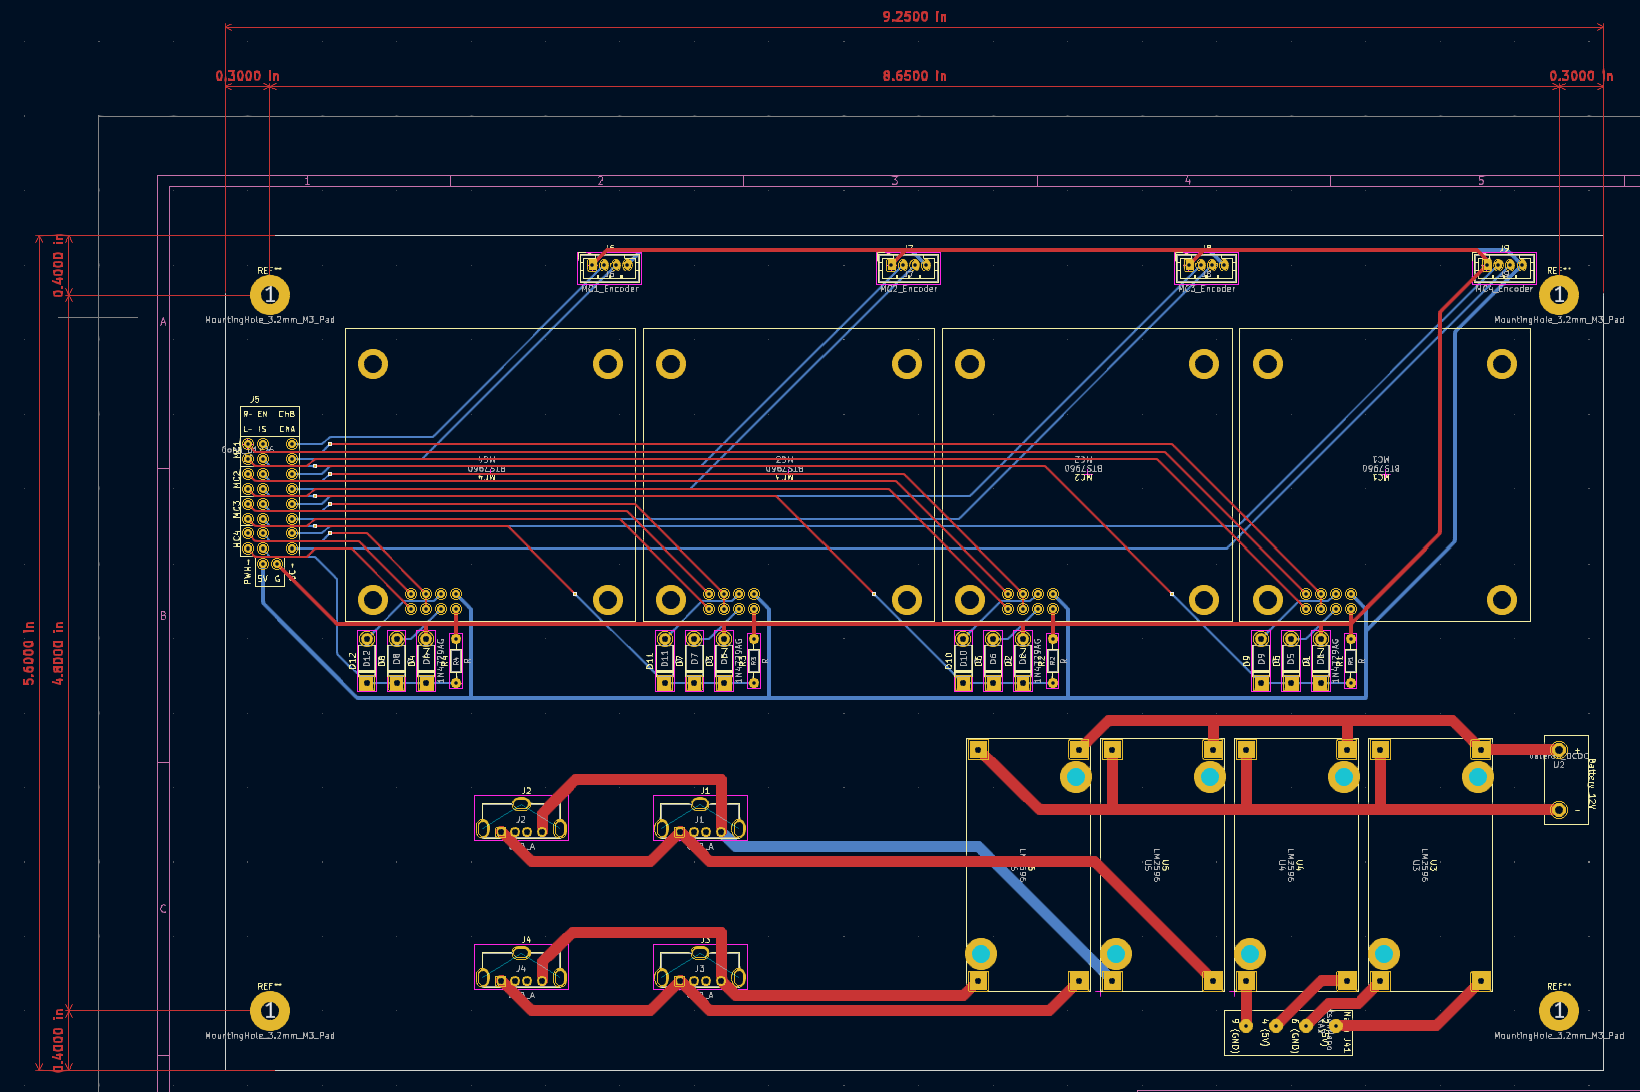
\includegraphics[scale=0.15]{Photos/Rover PCB}

\begin{itemize}
\item
	The PCB is designed to distribute power to every electrical hardware from a single power source or battery. And as well as, provide the signal connections for the hardware as they are essential in controlling the functionality of every component.
\end{itemize}


\textbf{Arduino Mega}

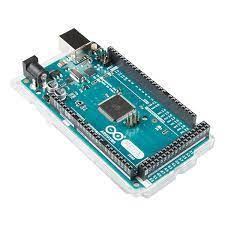
\includegraphics[scale=0.5]{Photos/Arduino Mega}

\begin{itemize}
\item
	Arduino Mega is a microcontroller that is designed to control the motors by controlling the motor controllers that control the drivetrain.
\end{itemize}


\textbf{Jetson Nano}

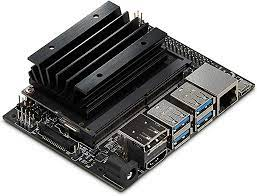
\includegraphics[scale=0.5]{Photos/Jetson Nano}

\begin{itemize}
\item
	The Jetson Nano is a small computer that is designed to run multiple neural networks like image processing, object detection, etc. 
\end{itemize}


\textbf{12V DC-DC Buck Converters}

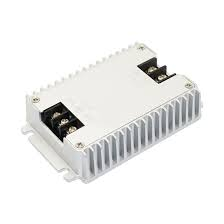
\includegraphics[scale=0.5]{Photos/12V DC-DC buck converter}

\begin{itemize}
\item
	The 12V DC-DC buck converter is used to step down any voltage larger than 12V down to its assigned level of 12V.
\end{itemize}


\textbf{LM2596 Buck Converters}

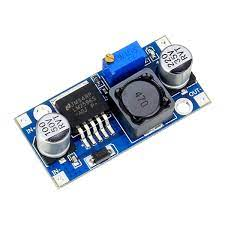
\includegraphics[scale=0.5]{Photos/LM2596 bucks}

\begin{itemize}
\item
	The LM2596 buck converters are designed to step down or drop down the voltage that is needed by the electrical components to be able to functionally run. And it's adjusted by a potentiometer that controls the voltage level output.
\end{itemize}


\textbf{BTS7960 Motor Controller}

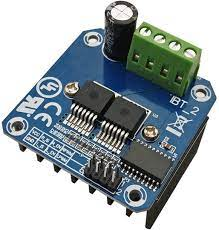
\includegraphics[scale=0.5]{Photos/BTS7960 Motor Driver}

\begin{itemize}
\item
	The motor controller is used to receive signals from the Arduino Mega and delivers it to the actual motors of the drivetrain.
\end{itemize}

\textbf{12V Planetary Gear Motors}

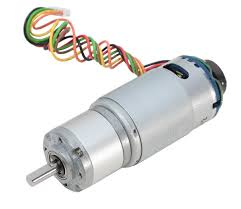
\includegraphics[scale=0.5]{Photos/Gear motor 12V planetary}

\begin{itemize}
\item
	The 12V planetary motors are used to drive the whole rover which are controlled by the BTS7960 motor controller through digital signals from the Arduino Mega.
\end{itemize}

\underline{Risk identification}

\begin{itemize}
\item
	One of the major risks or dangers for the electrical system is the probability of overheating which will cause a fire hazard. This will cause permanent damage to many of the components on the rover. The battery and the components that needed the most power are at risk of this danger, so sufficient protection for these parts will lower the risk of this danger.

\item
	The risk of the motors running too much or insufficient torque will cause different amounts of currents to be drawn from the battery. This current spike will cause damage to the electrical hardware that is directly connected to the battery and cause a fire hazard. The mechanical components will also face damage as a result.
\end{itemize}

\underline{Software System}


		\subsubsection{Electrical}
		The electrical circuit or model will be tested with the mechanical models, and the approximate date of testing will take place from the end of April to May. Testing will involve making sure connections are stable and all electrical components are functioning correctly and correspondingly communicate with each other. 
		
Future testing of electrical components and their functions:
\begin{itemize}
\item
The connections between components

\item
PCB functionality

\item
Jetson Nano connection

\item
Arduino Mega and Drivetrain connection

\item
Battery and power/current performance
\end{itemize}

The main risk of the electrical circuit or model is that the electrical connection between any electrical components has failed. The risk mitigation can involve:

\begin{itemize}
\item
Rewiring/replacing wires, checking every connection between every electrical component.

\item
Replacing old/faulty components with new ones can decrease the risk of circuit failure.
\end{itemize}

Another risk of the electrical circuit is the uneven distribution of power to any electrical component through voltage/current spikes and voltage/current noise. The risk mitigation can involve:

\begin{itemize}
\item
Adding new electrical components that are used to mitigate or decrease voltage/current spikes.

	\begin{itemize}
		\item
		Snubber diodes, bypass capacitors, transistors, and any other component that can prevent undesirable effects. 
	\end{itemize}
	
\item
Adding fuses can be used as a fail-safe to prevent the failure of the entire electrical system.
\end{itemize}


Another risk is any wire disconnecting during a test run which can cause an open circuit with the current not flowing in the intended direction and flowing towards volatile electrical components. The risk mitigation can involve:

\begin{itemize}
\item
Adding new electrical components that are used to block current.

	\begin{itemize}
		\item
		Blocking diodes and transistors can protect volatile components by preventing or blocking current from flowing backwards to a vulnerable component. 
	\end{itemize}
\end{itemize}

Future risks will be identified with further testing of the models.

		
		
----------------------------------HUH!?


\section{Methodology}
	\subsection{Mechanical}
		\subsubsection*{Early Motor Selection}
		The lack of documentation from previous year's teams, and the dearth of UWB mechanical design education makes designing a rover hard or almost impossible. I scraped through websites, forums, and catalogs of books to try and find the best I can on rover design and drive train design. 
	
		Since the motor dictates the design we had to get its data sheet. All literature advises over-sizing motors and running them at 10-20\% their stall torque in continuous run, split the difference and we should be working at 15\%; further analysis will get a more precise value. This makes sense as maximum efficiency occurs roughly at 15\% stall torque; we want to minimize battery drain. Doing this will set both the speed and torque output, the latter which will determine the weight of the rover. We don't expect the first iteration to drive up stairs, but when future iterations do, the incline increases net torque experienced; still we hope this won't creep up past 20\%. Obvious future changes could be to accept normal operating torque of 10\% of stall after reducing weight. The calculations for experienced forces driving up stairs in extreme conditions and on flat terrain still need to be completed at this stage.
		
		The operation of the motor is also intimately related to travel speed and power consumption. We must determine early if the planetary gear motors provided by RobotZone have already considered losses to inefficiencies of gears, and how that will affect power consumption, but not sure this is possible. The rover travel speed is based on the diameter and angular speed of the tank drive sprocket. The angular speed of the tank drive sprocket is the motor's angular speed, which is not actually 612RPM, despite being named so. Remind yourself that 612RPM is the no-load speed (this particular motor has 10\% uncertainty by the way) and this decreases linearly with increasing torque. Operating at 15\% torque we should actually expect to see 520RPM (85\% speed). I will soon create accurate (enough) motor curves for reference, and calculate exact parameters on torque experienced and maximum weight allowed. 
		
		\subsubsection*{Generating Motor Curves}
		Motor curves are simple plots of torque vs current, power, speed, and efficiency. Speed is inversely proportional to torque, with the maximum value being the no-load speed (written on the motor) occurring at 0 torque, and the minimum value being 0 at stall torque. We have two potential motors for use, so I'll generate the curves for both: 612RPM and 118RPM motors.
		
		The current has no-load and stall torque values; for our particular 612RPM (or 64.08 rads/sec) these are 0.5A (no-load) and 20A (stall). Mechanical power can be found as the product of torque (Nm) and angular velocity (rads/sec); this is different than electrical power, which is the product of applied voltage and drawn current. Efficiency is the ratio of mechanical power (output) to electrical power (input). Stall torque is 16kgF-cm, or about 1.57Nm.
		
		With the above parameters I used Desmos to plot the motor curve of our selected motor. Torque units are in Newton meters, rotational velocity (red line) units are in rads/sec, mechanical output power (green) are in Watts, current (blue) is in amps. The \textbf{efficiency (black) has been multiplied by a factor of 50} for easy visualization; correcting and we see a maximum of 31.25\% efficiency at $ 0.21/1.57 => 13.37\% $ of the stall torque.
		
		\begin{figure} [!h]
			\centering
			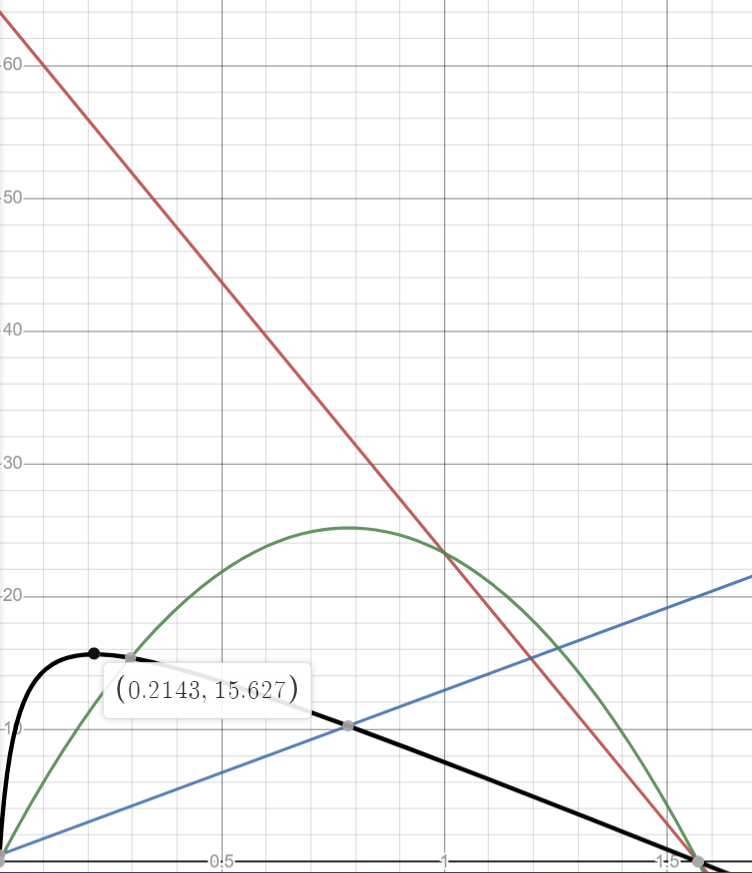
\includegraphics[scale=0.5]{Photos/motor_curves_612}
			\caption{Motor curves with efficiency multiplied by a factor of 50 for scale}
			\label{motor_curves_612}
		\end{figure}
		
		For our 118RPM (or 12.35 rads/sec) current values are 0.5A (no-load) and 20A (stall). Stall torque is 69kgF-cm, or about 6.76Nm. 
		
		With the above parameters I used Desmos to plot the motor curve of our selected motor. Torque units are in Newton meters, rotational velocity (red line) units are in rads/sec, mechanical output power (green) are in Watts, current (blue) is in amps. The \textbf{efficiency (black) has been multiplied by a factor of 20} for easy visualization; correcting and we see a maximum of 26.05\% efficiency at $ 0.927/6.79 = 0.1365 => 13.65\% $ of the stall torque. 
		
		\begin{figure} [!h]
			\centering
			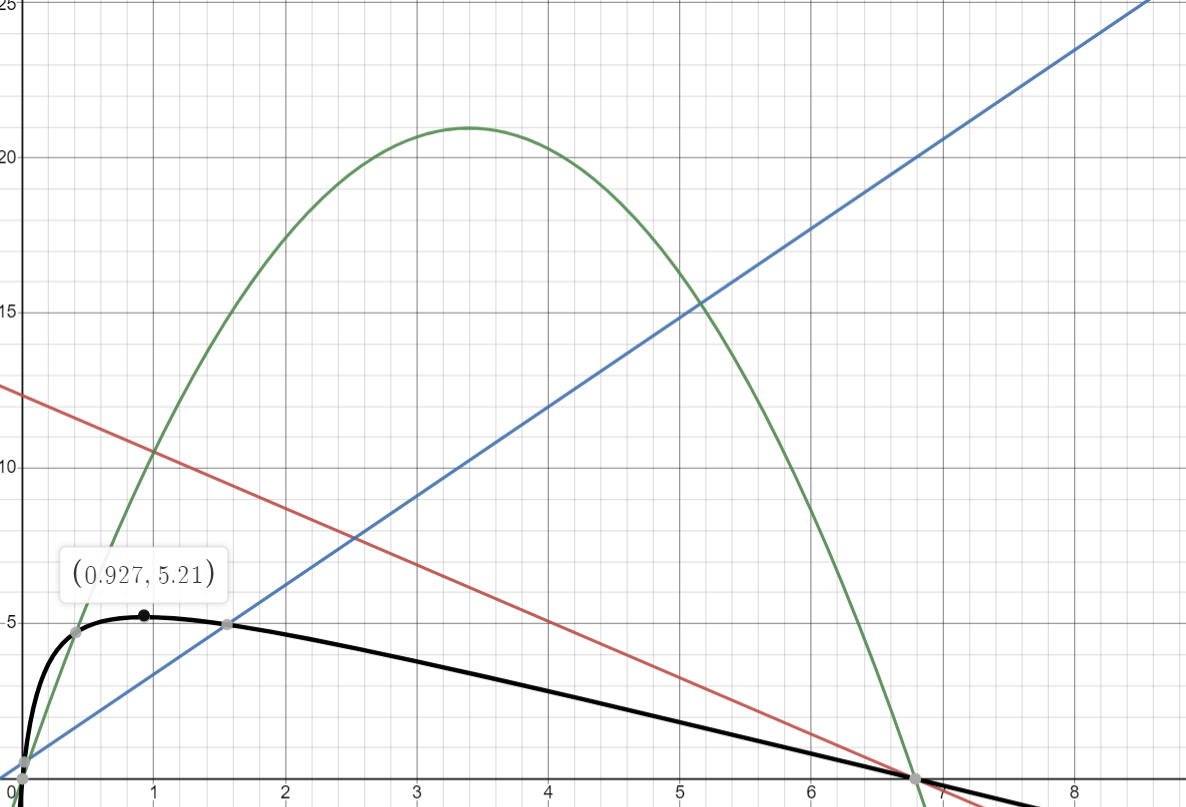
\includegraphics[scale=0.5]{Photos/motor_curves_118}
			\caption{Motor curves with efficiency multiplied by a factor of 20 for scale}
			\label{motor_curves_118}
		\end{figure}

		\subsubsection*{Determining torque, maximum allowable size, and speed}
		See the motor curves above for useful context. When considering the 612RPM motors, we've determined a maximum efficiency of 31.25\% if we run the motor at 13.37\% of the stall torque, which is about 0.214Nm. 
		
		At 13.37\% of the stall torque, we'd be running 86.63\% of the no-load speed, or 526RPM, which is 55 rads/sec. The velocity of a tank tread is simply the linear velocity of it's drive sprocket. The current design, which we're building on uses 2400 Series goBUILDA tracks, and a 100mm diameter sprocket; thus linear velocity is $v = 55rad/s * 50mm$, a reasonable 2.75 meters per second, or a little over 8 feet per second. 
		
		If we assume we're going to drive this rover entirely flat at the maximum efficiency, our motor should experience 0.214Nm of torque. When moving a single 50mm radius sprocket, the force developed at the contact is 4.28 Newtons. From here things are a bit confusing, as from first glance the rover appears to have two of these motors, but the document (which is admittedly outdated) shows 4. If we have 2 our total force propelling the rover is 8.56 Newtons, 4 and it's 17.l2 Newtons. Move past the motors for a moment and determine what our rover must overcome to move. Consulting some literature, a liberal frictional coefficient for tread based vehicles should be 0.5 the weight; 0.7 will be our conservative. I'm also going to do the calculations for the rubber tank treads we might use in the future at 0.9 (around the value of rubber on dry concrete). The tank treads never roll, so static friction is a constant. The force to overcome is thus 
		$$F_{app} = \mu mg$$
		We can assume that the motor will match this force, and solve for the only unknown (our mass). If we assume two motors outputting 8.56 Newtons: at the liberal friction coefficient estimate our ideal weight should be 1.75kg (3.8lbs), while for the conservative it should be 1.25kg (2.75lbs), and the future rubber treads about 0.97kg (2.13lbs). Obviously this is a massive weight reduction from the current 25 lbs rover, which would cause the motors to deliver 88\% its stall torque, an incredible inefficiency. I really want my math to be wrong, but nothing from their MegaDoc explains the decisions they made. If we assume 4 motors and 17.12 Newtons, then the ideal weight should be liberal - 3.5kg (7.9lbs), conservative - 2.5kg (5.5lbs), and future - 1.94kg (4.26lbs); again this is a huge difference from the realistic 25 lbs rover, which would require the motors to deliver 44\% its stall torque. Remember, our goal is 13\%... Trying to read back through their document I see mention of a speed test, but they placed the data into an image that got corrupted and never submitted with the PDF. There is one mention I saw of 1.1m/s, and while I don't think it's the rover they built, it would correspond to about 70\% of stall torque, causing me to lean on the side of 2 motors. I think what happened was this last team wanted a faster rover, and mindlessly piggybacked off the year-prior team's decision to use 118RPM motors without considering the torque specifications of the rover. If that rover uses 2 motors instead of 4, it's damn near a miracle it works, and it certainly wouldn't work climbing stairs. 
		
		The guaranteed takeaways are: (1) we need to drastically reduce the weight as much as possible to reach peak efficiency, or (2) we need to swap out the motors for 118RPM motors which will result in improved efficiency, and possibility to climb stairs. Fortunately most of the logical components don't amount to collectively more than a pound, leaving between 4 and 6 pounds for the rest of the chassis, batteries, and Stewart platform. 
	
		Another future consideration is performance on stairs. The equation used above was flat only, however it would become 
		$$F_{app} = \mu mgsin\theta + mgcos\theta$$
		for traveling up an incline of $\theta$ degrees. The increase here is appreciable when you consider how steep Discovery Hall's stairs are. Even 4 612RPM motors would be pushing their luck, we'd prefer 4 118RPM motors. 
		
		There are two situations that follow from this point: we continue running the two 612RPM motors, or swap out for 118RPM motors. Assuming we go with two 612RPM we see:
		\begin{itemize}
			\item Close to 88\% stall torque in continuous operation at \textbf{current weight}
			\item Efficiency of 5\% in continuous operation at \textbf{current weight}
			\item Increasing efficiency to 31.25\% as we reduce from 25lbs to 3lbs
			\item Increasing speed to 526RPM and 2.75 meters per second as we reduce from 25lbs to 3lbs.
		\end{itemize}
		The current speed given the torque should be 12\% of the max speed, or 73.44RPM (7.69 rads/sec), which corresponds to 0.38m/s. Their recorded value of 1m/s corresponds more closely to 30\% of the max speed, but it's still hard to believe.
		
		If we choose to swap out the 118RPM motors, at an ideal weight we'll be putting out 13.65\% of the stall torque and attaining 26.05\% efficiency. For this scenario we have the three friction coefficients: (1) liberal - 0.5, (2) conservative - 0.7, (3) alternative rubber treads for the future - 0.9. A single motor will develop 0.923Nm of torque, and on 50mm radius sprockets, this translates to 18.46Nm of force, for a 2 motor applied force of 36.92N. Ideal weights are thus liberal - 7.53kg (16.6lbs), conservative - 5.37kg (11.8lbs), and alternative - 4.18kg (9.21lbs). In our current scenario we assume 25lbs (11.3kg), resulting in a required force of 55.4N between two motors, or an experienced torque of 1.38Nm, which is pleasing 20.4\% of the stall torque, and efficiency of 25.29\%. This 25.29\% is extremely close to the ideal efficiency of 26.05\%. On the other end of the extreme, with rubber treads and 0.9 friction coefficient,  we need 2.49Nm of torque, which is an alright 36.7\% of the stall torque, and efficiency of 21\%. This corresponds to a liberal speed of 0.49m/s, or conservative speed of 0.39m/s. 
		
		So what we see if we swap out the 612RPM motors for 118RPM motors is a mild decrease in speed, and massive increase in efficiency. At this current stage it makes the most sense to swap out motors and drop the weight. If we're able to drop the weight significantly we can go back to 612RPM motors. 
		
		\subsubsection*{Testing Speed and Efficiency}
		Knowing now that we've decided upon 2 118RPM motors, and implemented them, we must conduct tests. As the analysis shows above, for a 25lbs rover we should expect, conservatively 0.39m/s of speed. Conducting a speed test would grant insight into the efficiency and operating conditions of the motor. In figure ----INSERT REFERENCE were the results of our test.
		
		-----INSERT IMAGE OF TEST'
		
		
		
		





Electrical:

The data that we need to collect involves current/power performance when the puzzle panel power distribution system and the entire rover operates. And also, the duration the batteries can last under a full operation by measuring the rate of the current. A special tool called a Clamp Meter is used to measure current values in real time. And it also, doesn't require wire to wire connection to measure as Clamp Meter measures through the magnetic fields from where the current is present. Acquiring the current measurements help determines the overall performance of the rover, its battery life and overall efficiency.

The industry standards used, is the usage of a professional PCB design program KiCad EDA which famous companies known for inventing Electrical Engineering projects like Adafruit which is known to design arduinos which are used in this project, Digi-Key Electronics which is known to manufacture standardized and basic electrical components, most are utilized to create the power distribution PCB of the rover.

\section{Results and Discussion}

Electrical:

The testing for the results in measuring current performance and voltage leveling accuracy in the puzzle panel power distribution system was a success. Demonstrating the test, we utilized a stationed multimeter to measure and monitor the output voltage in the picture below. 

%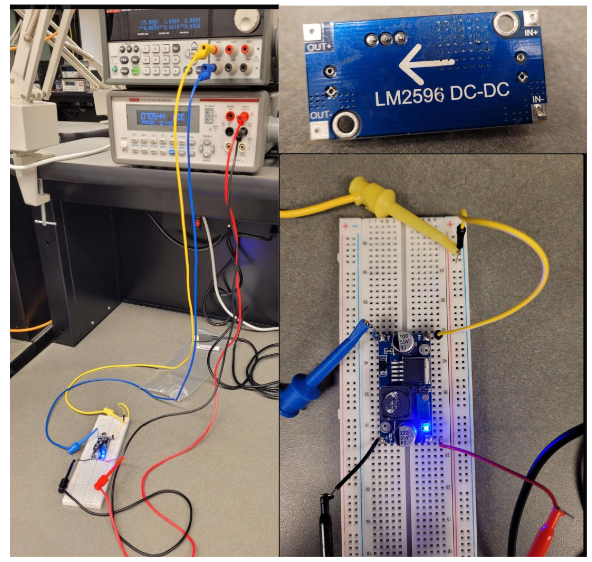
\includegraphics[scale=0.7]{Photos/LM2956 Testing Picture}

We tested every buck converter with this method. There were many that are broken down which we discarded in the waste box, but we desoldered some of the components which we can save for a different project. The ones we found to work, we used them for the final design of the Puzzle Panel power distribution system and for the rover PCB. In the table below, illustrates the results of one of the buck converters working well with a high input voltage and being able to step it down to any voltage lower than the input. And also, it is able to output the stepped down voltage which is essential in powering some of the hardware we have that requires low level voltage. There is a table with more data in terms of current and power performance in the Appendices and Supplement Data Section of this Megadoc and in the Electrical test report of the Buck Converter.

%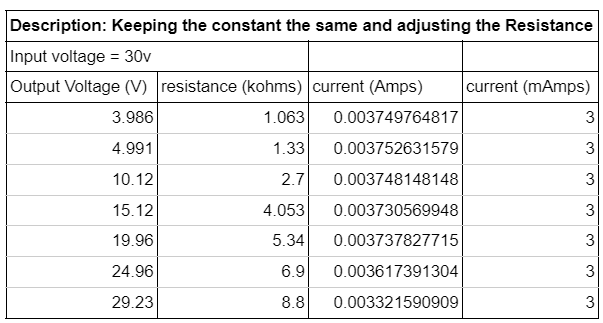
\includegraphics[scale=0.8]{Photos/Buck Converter Test Result}

After getting the buck converters to work, we soldered them onto the puzzle panel PDS. And we then powered the whole PDS to provide power to the actual Puzzle Panel elements which is shown below. 

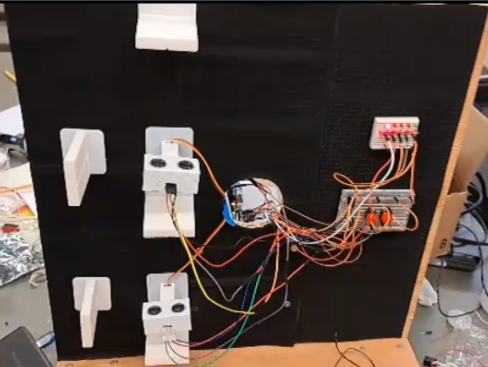
\includegraphics[scale=0.85]{Photos/Puzzle Panel Powered}

We then monitored the power efficiency and delivery of the Puzzle Panel PDS to the puzzle panel elements. The results showed it was successful. Every buck module are able to output the specified voltage based on the adjustment of their potentiometers. And when powering the hardware and the puzzle panel elements, there were no signs of electrical failures. The most number of elements that are connected to the PCB are three and when they operate, they draw 0.3A to 0.5A. With other slots of power and USBs in the PCB that are available, additional hardware or puzzle elements can be powered from the PCB. And with the performance of power not showing signs of failure, we can safely assume the Puzzle Panel PCB can handle powering multiple hardware and components at once.

The testing for the results in measuring the current/power performance of the rover are successful. We monitored the current levels going into the motor controllers running at 12V during a simple operational maneuver and the rover used around 1.5A when operating on flat ground. The next test involve operating the rover on dirt ground and driving over uneven terrain. Introducing dirt and uneven terrain would require the rover to draw more current since dirt and uneven terrain cause friction and resistant force for the rover to overcome. The results of the tests are successful with the rover operating over dirt in 1.6A to 1.7A and for uneven terrain, around 2.0A was used. The next major test involve moving the rover against the wall, to test the rover when it meets a maximum physical force. The overall current level reached to 3.3A which is more than twice the amount the rover used normally. These values help determine how long the rover perform under each of these environmental conditions. Additionally, there were no electrical hardware failures through each test, which we can conclude that the entire circuit is protected from voltage/current spikes or wire disconnects. And the current used in these conditions, are less than expected so we can safely assume the rover can handle harsher terrain and conditions.

\section{Summary, Conclusion and Future Perspectives}
"Summary section (in bullet form)
key open actions and concerns
Future perspectives"

Electrical:

\begin{itemize}
\item
Rover PCB: Redesign the layout of the components to manage space for better wire to wire connections, selecting newer and improved components that are more efficient and easy to use. Also, replacing any faulty or old hardware to prevent fatal electrical failures or accidents. Add a switch on and off button to turn on the whole rover rather than plugging the batteries to power the rover, this would help prevent possible injury when plugging big electrical wires that transmits high current to make contact with the person handling it
.

\item
Puzzle Panel PCB: Redesign the layout of the board to provide many more different alternatives to power different range of hardware, and select newer components to improve maximum power efficiency.

\end{itemize}

\section{Acknowledgments}

\section{Bibliography} 

\section{Appendices and Supplement Data}  

\textbf{Electrical Data} :

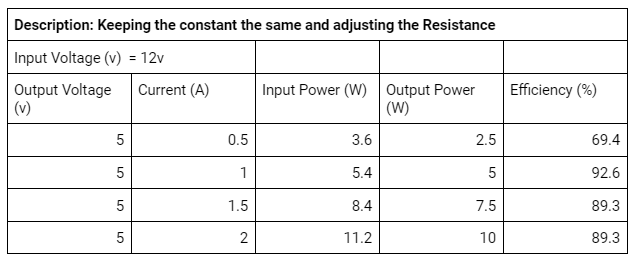
\includegraphics[scale=1.0]{Photos/Buck Converter Data}



\section{User Manual}

\textbf{Electrical User Manual:}

\textbf{IMPORTANT:} make sure no power source or battery is connected to any electrical system you are handling. Disconnect the battery or power away from the system to prevent electrical failures or accidents which may cause fatal injury and major damage to hardware.  

\textbf{Puzzle Panel} - The major components listed are, LM2596 buck converters and a female connector that receives power from a plugged in wall-wart.

1. To see how buck modules operate, its main function is to be able to take in a high level of voltage and output a different but lower level of voltage than the input. 

2. In both sides of the buck converters, they have positive and negative polarities. The negative pins of the converters are ground and the positive are actual power/voltage.  

3. To adjust the level, the LM2596 specifically have this resistant component called a potentiometer, its resistance is what determines how much voltage gets outputted. 

4. To monitor the output voltage, place a multimeter and have the positive lead connected to the positive output pin and the negative lead to the negative output pin. This tracks how much voltage is outputted and you can monitor how much voltage is being outputted after each adjustment.

5. Lowering the resistance, increases voltage output. And increasing resistance, decreases the output voltage. 

6. When using the Puzzle Panel Power distribution system, it's best to use a singular power source. For example, we used a 14.8V wall-wart and different rows of buck converters are adjusted to output, 3.3V, 5V, and 12V.

\textbf{Rover} - To setup the hardware, we'll start with the power connections before the digital connections.

1. Power connections need both positive and negative polarities to complete a circuit. First, the motor controllers needed positive and ground connections to be powered in B+ and B- slots. The M+ and M- indicate the polarities to connect to the actual planetary motors. 

2. Then, connecting the power to the hardware of the Jetson Nano, is by utilizing two separate jumper wires that power the Nano by 5V with two additional wires that are negative in respect to their positive counterparts.  

3. The Arduino Mega will be powered through a USB port that is built into the Power distribution PCB.

4. The LiDAR will receive power from the Nano through USB port in the Nano.

5. Next, onto the digital connections. The digital connections from the Motor Controllers are built into the PCB. To connect them to the Arduino Mega, jumper wires are utilized. And the labels and which ports to connect to on the Mega is shown in this diagram below.

%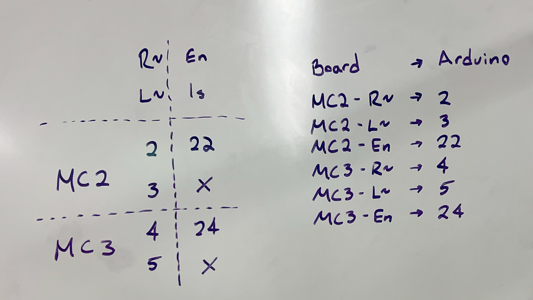
\includegraphics[scale=0.6]{Photos/Digital Connections from Motor Controller to Arduino Mega}

6. From the figure above, this allows the code of the software that is built into the Arduino Mega to communicate with the Motor controllers.

7. \textbf{IMPORTANT}: misplacing a digital wire connection can lead to severe consequences when giving a directional command to the rover. It can lead to hardware failure or operational accidents. So make sure the connection of each wire is correct and secure to prevent a disconnect when the rover operates.


\end{document}